%% This Beamer template is based on the one found here: https://github.com/sanhacheong/stanford-beamer-presentation, and edited to be used for Stanford ARM Lab

\documentclass[10pt]{beamer}
%\mode<presentation>{}

\usepackage{media9}
\usepackage{amssymb,amsmath,amsthm,enumerate}
\usepackage{mathtools}
\usepackage[utf8]{inputenc}
\usepackage{array}
\usepackage[parfill]{parskip}
\usepackage[utf8]{vietnam}
\usepackage{graphicx,animate}
\usepackage{caption}
\usepackage{subcaption}
\usepackage{bm}
\usepackage{amsfonts,amscd}
\usepackage[]{units}
\usepackage{listings}
\usepackage{multicol}
\usepackage{multirow}
\usepackage{tcolorbox}
\usepackage{physics}
\usepackage{movie15}
% Enable colored hyperlinks
\hypersetup{colorlinks=true}

\usefonttheme{professionalfonts}

% The following three lines are for crossmarks & checkmarks
\usepackage{pifont}% http://ctan.org/pkg/pifont
\newcommand{\cmark}{\ding{51}}%
\newcommand{\xmark}{\ding{55}}%

% Numbered captions of tables, pictures, etc.
\setbeamertemplate{caption}[numbered]
\usepackage{media9} 
%\usepackage[superscript,biblabel]{cite}
%\usepackage{algorithmic}
%\usepackage{algorithm2e}
%\usepackage{algpseudocode}
\usepackage[linesnumbered,ruled,vlined]{algorithm2e}
%\usepackage{algorithm}
%\usepackage{algorithmic}
%\usepackage{caption}
\usepackage[font=scriptsize,justification=centering]{caption}
%\usepackage{xcolor}
\usepackage{array}
%\renewcommand{\thealgocf}{}

\usepackage[natbib,backend=biber,style=ieee, sorting=ynt]{biblatex}
\bibliography{ref.bib}

\usepackage[acronym]{glossaries}

\usepackage{graphicx}
\graphicspath{{./figures}}
\usepackage{hyperref}

\usepackage{pythonhighlight}

\setbeamertemplate{theorems}[numbered]
\theoremstyle{remark}
\newtheorem{dl}{Định lý}
\newtheorem{md}{Mệnh đề}
\newtheorem{bd}{Bổ đề}
\newtheorem{dn}{Định nghĩa}
\newtheorem{hq}{Hệ quả}
%\theoremstyle{definition}

\numberwithin{algocf}{section}
\numberwithin{equation}{section}
\numberwithin{dl}{section}
\numberwithin{figure}{section}


%\newcommand{\empy}[1]{{\color{darkorange}\emph{#1}}}
%\newcommand{\empr}[1]{{\color{cardinalred}\emph{#1}}}
%\newcommand{\examplebox}[2]{
%\begin{tcolorbox}[colframe=darkcardinal,colback=boxgray,title=#1]
%#2
%\end{tcolorbox}}

%\usetheme{Stanford} 
%\input{./style_files_stanford/my_beamer_defs.sty}
\usetheme{Copenhagen}
\usecolortheme{seahorse}
%\logo{
\includegraphics[height=0.5in]{logos/HUS-name.jpg}}

\makeatletter
\let\@@magyar@captionfix\relax
\makeatother

\title[Kiến trúc lập trình song song và phân tán]{Kiến trúc lập trình song song và phân tán với OpenMP - MPI - CUDA}

\AtBeginSection[]
{
    \begin{frame}[shrink]
        \frametitle{Nội dung}
        \tableofcontents[currentsection, subsectionstyle=show/show/hide]
    \end{frame}
}

\setbeamertemplate{page number in head/foot}[totalframenumber]
\setbeamertemplate{frametitle continuation}{}

\begin{document}
\nocite{*}
\author[Nguyễn Chí Thanh - 21007925]{
	\begin{tabular}{c} 
	\Large
	Nguyễn Chí Thanh \\
    \footnotesize \href{mailto:nguyenchithanh\_sdh21@hus.edu.vn}{nguyenchithanh\_sdh21@hus.edu.vn}
\end{tabular}
\vspace{-4ex}}

\institute{
	\vskip 5pt
	\begin{figure}
		\centering
		\begin{subfigure}[t]{0.5\textwidth}
			\centering
			
\includegraphics[height=0.75in]{logos/HUS-logo.jpg}
		\end{subfigure}%
		~ 
		\begin{subfigure}[t]{0.5\textwidth}
			\centering
			
\includegraphics[height=0.75in]{logos/MIM-logo.png}
		\end{subfigure}
	\end{figure}
	\vskip 5pt	
	Đại học Quốc Gia Hà Nội \\
	Trường đại học Khoa học tự nhiên\\
	Khoa Toán - Cơ - Tin học
	\vskip 3pt
}

%\begin{noheadline}
\begin{frame}[shrink] \maketitle \end{frame}
%\end{noheadline}
    
\setbeamertemplate{itemize items}[default]
\setbeamertemplate{itemize subitem}[circle]

\begin{frame}{Nội dung}
    \tableofcontents[hidesubsections]
\end{frame}

\section{OpenMP}

\begin{frame}{Giới thiệu OpenMP}
    \begin{itemize}
        \item OpenMP là một API viết các ứng dụng đa luồng bộ nhớ chia sẻ sử dụng ngôn ngữ C/C++ hoặc Fortran
        \item Gồm có các chỉ thị biên dịch, runtime routine, biến môi trường.
        \item Hội đồng phát triển và phê duyệt kiến trúc OpenMP:
        \begin{itemize}
            \item Duy trì spec OpenMP
            \item Thành viên chính: AMD, Cray, Fujitsu, HP, IBM, Intel, Oracle, NVIDIA, Microsoft, Tesxas Instruments, Convey
            \item Thành viên ngắn hạn: ANL,	ASC/LLNL, cOMPunity, EPCC, LANL, NASA, TACC, RWTH, Aachen University, UH
        \end{itemize}
    \end{itemize}
\end{frame}

\begin{frame}{Các thành phần của OpenMP}
    \begin{columns}[onlytextwidth]
        \begin{column}{0.3\textwidth}
            Các chỉ thị biên dịch:
            \begin{itemize}
                \item Parallel region	
                \item Worksharing constructs
                \item Tasking
                \item Offloading
                \item Affinity
                \item Error Handling
                \item SIMD
                \item Synchronization
                \item Data-sharing attributes
            \end{itemize}
        \end{column}
        \begin{column}{0.3\textwidth}
            Các biến runtime:
            \begin{itemize}
                \item Số luồng
                \item Thread ID 
                \item Dynamic thread adjustment
                \item Nested parallelism
                \item Schedule
                \item Active levels
                \item Thread limit
                \item Nesting level
                \item Ancestor thread
                \item Team size 
                \item Locking
                \item Wallclock timer
            \end{itemize}
        \end{column}
        \begin{column}{0.3\textwidth}
            Các biến môi Trường:
            \begin{itemize}
                \item Số luồng
                \item Scheduling type
                \item Dynamic thread adjustment
                \item Nested parallelism
                \item Stacksize
                \item Idle threads
                \item Active levels
                \item Thread limit
            \end{itemize}
        \end{column}
    \end{columns}
\end{frame}

\begin{frame}
    \begin{figure}[H]
        \centering
        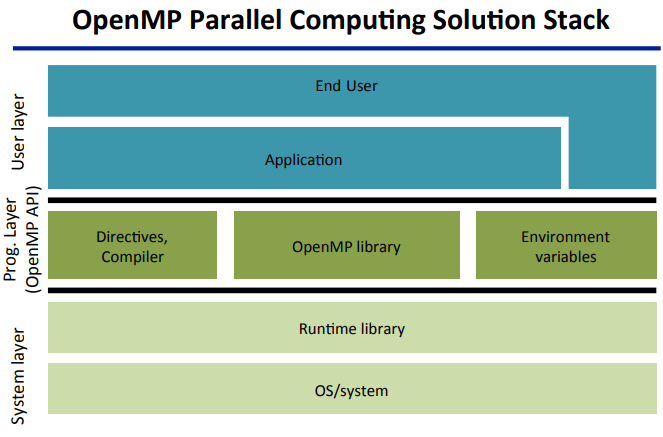
\includegraphics[width=0.9\linewidth]{figures/OpenMP/OpenMP_Parallel_Computing_Solution_Stack.png}
        \caption{Vị trí OpenMP trong stack}
    \end{figure}
\end{frame}

\begin{frame}{Chỉ thị biên dịch}
    \begin{itemize}
        \item Chỉ thị thực thi OpenMP áp dụng cho các khối có cấu trúc đứng kế tiếp với nó.
        \item Một chỉ thị bắt đầu với \#pragma omp. Các phần còn lại tuân theo quy ước của ngôn ngữ C và C++ cho các chị thị biên dịch 
    \end{itemize}
\end{frame}

\begin{frame}{Một số chỉ thị biên dịch của OpenMP}
    \begin{itemize}
        \item \#pragma omp parallel
        \item \#pragma omp for
        \item \#pragma omp sections
        \item \#pragma omp parallel shared/private
        \item \#pragma omp barrier
    \end{itemize}
\end{frame}

\begin{frame}{Mô hình thực thi Fork-Join của OpenMP}
    \begin{figure}[H]
        \centering
        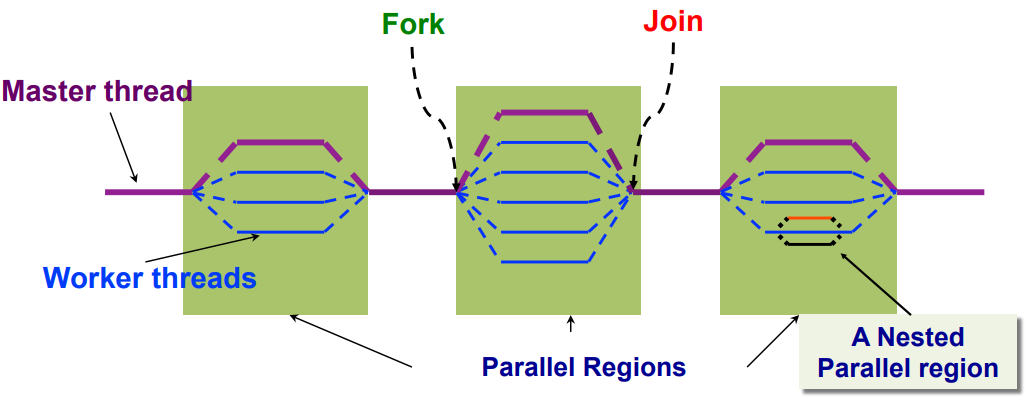
\includegraphics[width=\linewidth]{figures/OpenMP/Fork_Join_Execution_Model.png}
        \caption{Mô hình thực thi Fork-Join của OpenMP}
    \end{figure}
\end{frame}

\begin{frame}{Mô hình bộ nhớ của OpenMP}
    \begin{columns}[onlytextwidth]
        \begin{column}{0.5\linewidth}
            \begin{figure}[H]
                \centering
                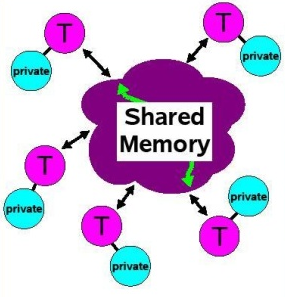
\includegraphics[width=\linewidth]{figures/OpenMP/OpenMP_Shared_Memory_Model.png}
            \end{figure}
        \end{column}
        \begin{column}{0.5\linewidth}
            \begin{itemize}
                \item Tất cả các luồng có cùng bộ nhớ chia sẻ toàn cục.
                \item Dữ liệu có thể chia sẻ hoặc riêng tư giữa các luồng
                \item Dữ liệu chia sẻ có thể truy cập từ tất cả các luồng
                \item Dữ liệu riêng tư chỉ có thể được truy cập từ luồng sở hữu dữ liệu
                \item Chia sẻ dữ liệu trong suốt với lập trình viên
                \item Có đồng bộ hóa, chủ yếu ngầm diễn ra.
            \end{itemize}
        \end{column}
    \end{columns}
    
\end{frame}

\begin{frame}[fragile]{OpenMP parallel region}
    Trong C/C++: một khối là một biểu thức hoặc một nhóm biểu thức giữa cặp ngoặc { }.
    \begin{columns}[onlytextwidth]
        \begin{column}{0.5\linewidth}
            \begin{verbatim}
#pragma omp parallel
{
    id = omp_get_thread_num();
    res[id] = lots_of_work(id);
}
            \end{verbatim}
        \end{column}
        \begin{column}{0.5\linewidth}
            \begin{verbatim}
#pragma omp parallel for
for(i=0;i<N;i++) {
    res[i] = big_calc(i);
    A[i] = B[i] + res[i];
} 
            \end{verbatim}
        \end{column}
    \end{columns}
\end{frame}

\begin{frame}{Chạy thực thi}
    \begin{itemize}
        \item Đặt biến môi trường OMP\_NUM\_THREADS.
        \item Chạy lệnh: g++ -fopenmp -g ./input.c -o ./input
    \end{itemize}
\end{frame}

\begin{frame}[shrink, fragile]{Chương trình đơn giản OpenMP}
    \begin{verbatim}
        #include <stdio.h>
        #include <omp.h>

        int main(int argc, char** argv) {
            #pragma omp parallel
            {
                printf("Hello World\n");
            } // End of parallel region 
            return 0;
        }
    \end{verbatim}
    Thực thi chương trình:
    \begin{verbatim}
        g++ -fopenmp -g ./hello_openmp.c -o ./hello_openmp
        ./hello_openmp
    \end{verbatim}
\end{frame}

\begin{frame}[fragile]{Khối lệnh có cấu trúc}
    \begin{itemize}
        \item Khối lệnh có cấu trúc: Một điểm vào và một điểm ra.
        \item Trong C/C++: một khối lệnh là một câu lệnh đơn hoặc một nhóm các câu lệnh giữa các ngoặc.
    \end{itemize}

    \begin{columns}[onlytextwidth]
        \begin{column}{0.5\textwidth}
            \begin{verbatim}
#pragma omp parallel
{
id = omp_get_thread_num(); 
A[id] = big_compute(id);
}		
            \end{verbatim}
        \end{column}
        \begin{column}{0.5\textwidth}
            \begin{verbatim}
#pragma omp for
for (int i=0;i<N;i++) {
    res[i] = big_calc(i);
    A[i] = B[i] + res[i]; 
}
            \end{verbatim}
        \end{column}
    \end{columns}
\end{frame}

\begin{frame}[fragile]{Cách viết rút gọn chỉ thị}
    Hai cách viết sau là tương đương:
    \begin{columns}[onlytextwidth]
        \begin{column}{0.5\textwidth}
            \begin{verbatim}
int i;
double res[MAX];
#pragma omp parallel				
{
    #pragma omp for
    for (i=0;i< MAX; i++) {
        res[i] = huge();
    } 
}
            \end{verbatim}
        \end{column}
        \begin{column}{0.5\textwidth}
            \begin{verbatim}
int i;
double res[MAX];
#pragma omp parallel for					
for (i=0;i< MAX; i++) {
    res[i] = huge();
}
            \end{verbatim}
        \end{column}
    \end{columns}
\end{frame}

\begin{frame}[fragile]{Đặt số luồng thực thi}
    Cách 1:
    \begin{verbatim}
export OMP_NUM_THREADS=4
    \end{verbatim}
    Cách 2:
    \begin{verbatim}
omp_set_num_threads(4);
    \end{verbatim}
\end{frame}

\begin{frame}[fragile]{Minh họa quá trình chạy song song}
    \begin{columns}[onlytextwidth]
        \begin{column}{0.5\textwidth}
            \begin{verbatim}
...A... 
#pragma omp parallel
{
    foo(); /* ...B... */
}
...C... 
#pragma omp parallel
{
...D...
}
...E...
            \end{verbatim}
        \end{column}
        \begin{column}{0.5\textwidth}
            \begin{figure}[H]
                \centering
                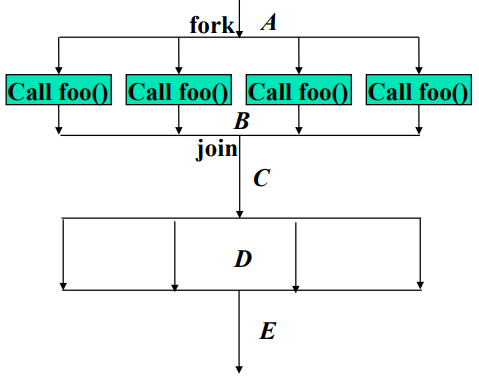
\includegraphics[width=\linewidth]{figures/OpenMP/Fork.png}
            \end{figure}
        \end{column}
    \end{columns}
\end{frame}

\begin{frame}[fragile]{Nguyên lý thiết kế}
    \begin{verbatim}
#pragma omp parallel
{
    int thread_id = omp_get_thread_num();
    int num_threads = omp_get_num_threads();
    printf("Thread %d of %d\n", thread_id, num_threads); 
}
    \end{verbatim}
    \begin{itemize}
        \item Từng hàm printf() là một tác vụ
        \item Parallel region tập hợp một tập các luồng cho tính toán và xử lý.
        \item Từng luồng thực thi một tác vụ đơn lẻ
        \item Ánh xạ 1:1 giữa các tác vụ và luồng
    \end{itemize}
\end{frame}

\begin{frame}[fragile]{Cú pháp OpenMP}
    \begin{itemize}
        \item OpenMP sử dụng các chỉ thị biên dịch dạng \#pragma.
        \item Với C và C++, chỉ thị có dạng:
        \begin{verbatim}
#pragma omp construct [clause [clause]...]
        \end{verbatim}
        \item Khai báo tệp tiêu đề: \#include <omp.h>
    \end{itemize}
\end{frame}

\begin{frame}[shrink, fragile]{Mô hình chương trình SIMD}
    \begin{itemize}
        \item SIMD cho parallel region:
        \begin{itemize}
            \item Tất cả các luồng của parallel region cùng thực thi một đoạn code.
            \item Mỗi luồng có một ID riêng
        \end{itemize}
        \item Có thể sử dụng threadID để phân nhánh thực thi các luồng, các luồng khác nhau có thể theo những con đường khác nhau qua cùng đoạn code:
        \begin{verbatim}
if(thread_id == x) {

} else {

}
        \end{verbatim}
        \item SIMD được sử dụng rất phổ biến cho cấu trúc các chương trình song song: OpenMP, MPI, CUDA,...
    \end{itemize}
\end{frame}

\begin{frame}[fragile]{Phân nhánh parallel regions}
    Chỉ có luồng master in ra màn hình số luồng
        \begin{verbatim}
#pragma omp parallel
 {
    int thread_id = omp_get_thread_num(); 
    int num_threads = omp_get_num_threads();
    if (thread_id == 0) 
        printf("Thread %d of %d\n", thread_id, num_threads); 
    else 
        printf("Thread %d\n", thread_id);
 }
        \end{verbatim}
\end{frame}

\begin{frame}[fragile]{Phân nhánh parallel regions}
    Chỉ có luồng master đọc số luồng và tất cả các luồng cùng in ra số luồng
    \begin{verbatim}
#pragma omp parallel
{
    int thread_id = omp_get_thread_num();
    if (thread_id == 0)
        num_threads = omp_get_num_threads();
    #pragma omp barrier
    printf("Thread %d of %d\n", thread_id, num_threads); 
}
    \end{verbatim}
\end{frame}

\begin{frame}{Chỉ thị Barrier}
    \begin{figure}[H]
        \centering
        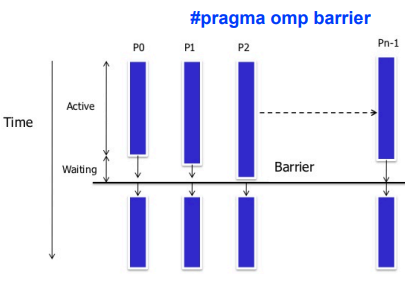
\includegraphics[width=0.9\linewidth]{figures/OpenMP/Barrier.png}
        \caption{Đồng bộ hóa giữa các luồng}
    \end{figure}
\end{frame}

\begin{frame}[shrink, fragile]{Chỉ thị Barrier}
    \begin{verbatim}
#pragma omp parallel shared (A, B, C) private(id)
{
    id=omp_get_thread_num();
    A[id] = big_calc1(id);
    #pragma omp barrier
    #pragma omp for
    for(i = 0;i < N; i++){
        C[i] = big_calc3(I, A);
    }
    // Có một barrier ngầm định kết thúc vòng lặp for
    #pragma omp for nowait // loại bỏ barrier
    for(i=0; i < N; i++){ 
        B[i] = big_calc2(C, i); 
    }
    A[id] = big_calc3(id);
} // Một barrier ngầm định kết thúc parallel region
    \end{verbatim}
\end{frame}

\begin{frame}[fragile]{Chỉ thị master}
    \begin{itemize}
        \item Ký hiệu khối lệnh chỉ được thực thi bởi luồng master
        \item Các luồng khác bỏ qua
        \item Không có đồng bộ hóa ngầm định
    \end{itemize}
    \begin{verbatim}
#pragma omp parallel private (tmp)
{
    do_many_things_together();
    #pragma omp master
    { 
        exchange_boundaries_by_master_only (); 
    }
    #pragma barrier
    do_many_other_things_together();
} 
    \end{verbatim}
\end{frame}

\begin{frame}[fragile]{Chỉ thị single}
    \begin{itemize}
        \item Ký hiệu khối lệnh chỉ được thực thi bởi một luồng
        \item Một barrier được ngầm định ở cuối khối lệnh
    \end{itemize}
    \begin{verbatim}
#pragma omp parallel private (tmp)
{
    do_many_things_together();
    #pragma omp single
    { 
        exchange_boundaries_by_one(); 
        }
    do_many_other_things_together();
}
    \end{verbatim}
\end{frame}

\begin{frame}[shrink, fragile]{Phân chia công việc sử dụng thread id}
    \begin{figure}[H]
        \centering
        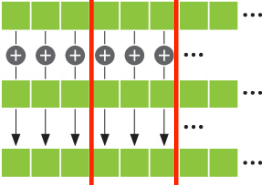
\includegraphics[width=0.3\linewidth]{figures/OpenMP/Distribute.png}
    \end{figure}
    \begin{verbatim}
        #pragma omp parallel shared (a, b)
        {
            int id, i, Nthrds, istart, iend;
            id = omp_get_thread_num();
            Nthrds = omp_get_num_threads();
            istart = id * N / Nthrds;
            iend = (id+1) * N / Nthrds;
            for(i=istart;i<iend;i++) { 
                a[i] = a[i] + b[i]; 
            }
        } 
    \end{verbatim}
\end{frame}

\begin{frame}[shrink, fragile]{Các mệnh đề schedule}
    Mệnh đề schdule được dùng để xác định cách chia vùng dữ liệu trong các vòng lặp giữa các luồng
    \begin{itemize}
        \item schedule (static | dynamic | guided [,chunk\_size])
        \item schedule (auto | runtime)
    \end{itemize}
    \begin{itemize}
        \item static chia các lặp lại của một vòng lặp thành các phần có kích thước bằng nhau và gán một phần cho mỗi luồng.
        Kích thước các phần được xác định tại thời điểm biên dịch và duy trì không đổi trong suốt quá trình thực thi của vòng lặp.
        \item dynamic gán các đoạn nhỏ của dữ liệu cho các luồng tại thời điểm chạy.
        Mỗi luồng thực hiện phần được gán và yêu cầu đoạn tiếp theo khi hoàn thành (các đoạn nhỏ kích thước bằng nhau).
        Kích thước các đoạn dữ liệu do từng luồng đảm nhận khác nhau.
        \item guided tương tự như dynamic nhưng các đoạn dữ liệu nhỏ do từng luồng đảm nhận giảm theo hàm mũ.
    \end{itemize}
\end{frame}

\begin{frame}[fragile]{Các mệnh đề schedule}

    \begin{itemize}
        \item auto cho phép OpenMP tự động chọn lịch trình phù hợp dựa trên điều kiện của runtime.
        Lịch trình được đưa ra bởi hệ thống.
        \item runtime cho phép lịch trình và chunk\_size xác định tại thời điểm chạy sử dụng biến môi trường.
    \end{itemize}
    \begin{verbatim}
#pragma omp parallel for schedule(static) private(id)
for(i = 0; i < N; i++) {
    A[i] = B[i] + C[i];
}
    \end{verbatim}
\end{frame}

\begin{frame}{Các mệnh đề schedule}
    \begin{figure}[[H]]
        \centering
        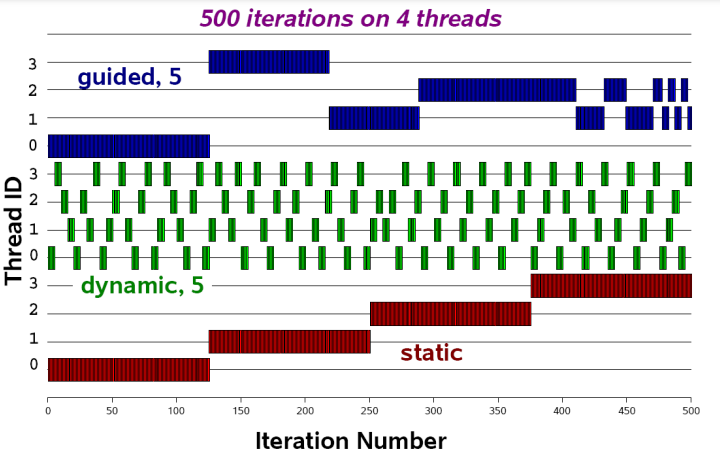
\includegraphics[width=0.8\linewidth]{figures/OpenMP/Schedule_Modes_Comparison.png}
        \caption{So sánh các chế độ schedule}
    \end{figure}
\end{frame}

\begin{frame}[fragile]{Chỉ thị sections}
    Mỗi section được gán cho một thread
    \begin{verbatim}
#pragma omp parallel
#pragma omp sections
{
    #pragma omp section
    printf("1 + 1, id: %d\n", omp_get_thread_num());
    #pragma omp section
    printf("1 + 2, id: %d\n", omp_get_thread_num());
    #pragma omp section
    printf("1 + 3, id: %d\n", omp_get_thread_num());
}
    \end{verbatim}

    Một barrier ngầm định ở cuối khối omp sections.
    Có thể tắt barrier sử dụng từ khóa nowait.
\end{frame}

\begin{frame}[fragile]{Chỉ thị sections}
    \begin{verbatim}
#pragma omp parallel private(id)
{
    int id = omp_get_thread_num();
    #pragma omp sections nowait
    {
        #pragma omp section
        printf("1 + 1, id: %d\n", id);
        #pragma omp section
        printf("1 + 2, id: %d\n", id);
        #pragma omp section
        printf("1 + 3, id: %d\n", id);
    }
    printf("%d\n", id);
}
    \end{verbatim}
\end{frame}

\begin{frame}[fragile]{Loop Collapse}
    \begin{itemize}
        \item Cho phép song song hóa giữa các vòng lặp lồng nhau mà không cần dùng song song hóa lồng nhau.
        \item Mệnh đề collapse chỉ thị bao nhiêu vòng lặp bị collapse
    \end{itemize}
    \begin{verbatim}
#pragma omp parallel for collapse(2)
for (i = 0; i < M; i++) {
    for (j = 0; j < P; j++) {
        int temp = 0;
        for (k = 0; k < N; k++) {
            temp += *(B + i * N + k) * *(C + k * P + j);
        }
        *(A + i * P + j) = temp;
    }
}
    \end{verbatim}
\end{frame}

\subsection{Môi trường dữ liệu}

\begin{frame}{Môi trường dữ liệu}
    \begin{itemize}
        \item Hầu hết các biến được chia sẻ giữa các luồng
        \item Các biến toàn cục, static mặc định là chia sẻ
        \item Các biến cục bộ trong hàm được gọi trong parallel region hoặc các biến được khai báo trong parallel region là riêng tư.
        \item shared, private, firstprivate, lastprivate?
    \end{itemize}
\end{frame}

\begin{frame}{Mệnh đề private}
    \begin{itemize}
        \item Mệnh đề private khai báo một biến là riêng tư đối với mỗi luồng trong một parallel region.
        \item Các biến riêng có các phiên bản riêng cho từng luồng và mỗi luồng hoạt động với bản sao riêng của biến đó.
        \item Giá trị ban đầu của một biến riêng tư không được xác định, vì vậy nó cần được khởi tạo rõ ràng ở trong luồng.
        \item Sau khi kết thúc parallel region, giá trị biến ban đầu được trở lại giá trị ban đầu trước khi thực hiện parallel region (chưa được khởi tạo????)
    \end{itemize}
\end{frame}

\begin{frame}{Mệnh đề firstprivate}
    \begin{itemize}
        \item Giống như private nhưng biến riêng tư được khởi tạo bằng giá trị ban đầu của biến ban đầu.
        \item Sau khi kết thúc parallel region, giá trị biến ban đầu được trở lại giá trị ban đầu trước khi thực hiện parallel region (chưa được khởi tạo????)
    \end{itemize}
\end{frame}

\begin{frame}{Mệnh đề lastprivate}
    \begin{itemize}
        \item Giống như firstprivate nhưng giá trị của biến ban đầu sau khi thực hiện parallel region được gán cho giá trị cuối cùng mà một biến riêng tư được gán trong khi thực hiện parallel region.
    \end{itemize}
\end{frame}

\begin{frame}[fragile]{Ví dụ private}
    \begin{verbatim}
int id = 0;
#pragma omp parallel private(id)
{
    id = omp_get_thread_num();
    printf("Thread id %d\n", id);
}
printf("Thread %d id\n", id);
    \end{verbatim}
\end{frame}

\begin{frame}[fragile]{Mệnh đề reduction}
    \begin{itemize}
        \item reduction dùng để thực hiện các phép toán trên một biến được chia sẻ trên nhiều luồng trong một parallel region.
        \item reduction kết hợp các giá trị của biến trên từng luồng và lưu trữ kết quả trên một biến duy nhất
        \item Hay sử dụng khi tính tổng, tích, max, min trên một tập các giá trị.
        \item Hay được sử dụng với vòng lặp for.
        \begin{verbatim}
#pragma omp parallel for reduction(operator: variable)
        \end{verbatim}
    \end{itemize}
\end{frame}

\begin{frame}[fragile]{Mệnh đề reduction}
    \begin{verbatim}
int i = 0;
#pragma omp parallel reduction(*:i)
{
    i=omp_get_num_threads();
    printf("%d\n", i);
} // 1 * 4 * 4 * 4 * 4
printf("result=%d\n", i); 
    \end{verbatim}
\end{frame}

\subsection{Đồng bộ hóa trong OpenMP}
\begin{frame}
    \begin{itemize}
        \item Đồng bộ hóa mức cao:
        \begin{itemize}
            \item critical
            \item atomic 
            \item barrier
            \item ordered
        \end{itemize}
        \item Đồng bộ hóa mức thấp
        \begin{itemize}
            \item flush
            \item locks
        \end{itemize}
    \end{itemize}
\end{frame}

\begin{frame}[shrink, fragile]{critical}
    \begin{itemize}
        \item critical chỉ cho phép một luồng duy nhất được thực thi một đoạn code tại một thời điểm
    \end{itemize}

    \begin{verbatim}
int shared = 0;
#pragma omp parallel
{
    int thread_id = omp_get_thread_num();
    #pragma omp for
    for (int i = 0; i < 100; i++) {
        #pragma omp critical
        {
            shared += 1;
            printf("Thread %d: Incrementing shared to %d\n", 
            thread_id, shared);
        }
    }
}
    \end{verbatim}
    
\end{frame}

\begin{frame}[fragile]{So sánh với single}
    \begin{verbatim}
#pragma omp parallel num_threads(3)
{
   foo();
   bar();
   ...
}
    \end{verbatim}
thread 0: ----< foo() >< bar() >----------->

thread 1: --< foo() >< bar() >------------->

thread 2: ---------< foo() >< bar() >------>
\end{frame}

\begin{frame}[fragile]{So sánh với single}
    \begin{verbatim}
#pragma omp parallel num_threads(3)
{
   #pragma omp single
   foo();
   bar();
   ...
}
    \end{verbatim}
    \begin{verbatim}
thread 0: ------[-------|]< bar() >----->

thread 1: ---[< foo() >-|]< bar() >----->

thread 2: -------------[|]< bar() >----->
    \end{verbatim}
\end{frame}

\begin{frame}[fragile]{So sánh với single}
    \begin{verbatim}
#pragma omp parallel num_threads(3)
{
   #pragma omp single nowait
   foo();
   bar();
   ...
}
    \end{verbatim}
    \begin{verbatim}
thread 0: ------[]< bar() >----------->

thread 1: ---[< foo() >]< bar() >----->

thread 2: -------------[]< bar() >---->
    \end{verbatim}
\end{frame}

\begin{frame}[fragile]{So sánh với single}
    \begin{verbatim}
#pragma omp parallel num_threads(3)
{
   #pragma omp critical
   foo();
   bar();
   ...
}
    \end{verbatim}
    \begin{verbatim}
thread 0: ------xxxxxxxx[< foo() >]< bar() >-------------->

thread 1: ---[< foo() >]< bar() >------------------------->

thread 2: -------------xxxxxxxxxxxx[< foo() >]< bar() >--->
    \end{verbatim}
\end{frame}

\begin{frame}[shrink, fragile]{So sánh với single}
    \begin{verbatim}
#pragma omp parallel num_threads(3)
{
   if (omp_get_thread_num() > 1) {
     #pragma omp critical(foo2)
     foo();
   }
   else {
     #pragma omp critical(foo01)
     foo();
   }
   bar();
   ...
}
    \end{verbatim}
    \begin{verbatim}
thread 0: ------xxxxxxxx[< foo() >]< bar() >---->
thread 1: ---[< foo() >]< bar() >--------------->
thread 2: -------------[< foo() >]< bar() >----->
    \end{verbatim}
\end{frame}

\begin{frame}[fragile]{So sánh với single}
    \begin{verbatim}
#pragma omp parallel num_threads(3)
{
   #pragma omp critical
   foo();
   ...
   #pragma omp critical
   bar();
   ...
}
    \end{verbatim}

    \begin{verbatim}
0: ------xxxxxx[<foo()>]< ... >xxxxxxxxxxx[<bar()>]---------->
1: ---[<foo()>]< ... >xxxxxxxxxxx[<bar()>]------------------->
2: -------------xxxxxxxx[<foo()>]< ... >xxxxxxxxxxx[<bar()>]->
    \end{verbatim}
\end{frame}

\begin{frame}[fragile]{atomic}
    \begin{itemize}
        \item atomic là một trường hợp đặc biệt của critical sử dụng cho một số câu lệnh đơn giản
    \end{itemize}

    \begin{verbatim}
int thread_id = omp_get_thread_num();
//#pragma omp for
for (int i = 0; i < 100; i++) {
    #pragma omp critical
    shared += 1;
    printf("Thread %d: Incrementing shared to %d\n", thread_id, shared);
}
    \end{verbatim}
\end{frame}

\begin{frame}[fragile]{ordered}
    \begin{itemize}
        \item ordered bắt buộc vòng lặp thực hiện theo đúng thứ tự trong một parallel region
        \item Đảm bảo các vòng lặp hoặc các đoạn code thực hiện theo đúng thứ tự đưa ra bởi lập trình viên
    \end{itemize}
    \begin{verbatim}
#pragma omp parallel num_threads(4) private(tmp)
#pragma omp for ordered
for (int i = 0; i < 100; i++) {
    tmp = do_in_parallel(i);
    #pragma omp ordered
    printf("i: %d, thread id: %d\n", i, omp_get_thread_num());
}
    \end{verbatim}
\end{frame}

\begin{frame}[fragile]{locks}
    \begin{itemize}
        \item Chỉ cho phép một luồng thực thi một đoạn code tại một thời điểm.
        \item Ngăn khả năng bị race conditions khi nhiều luồng cố gắng truy cập và sửa một dữ liệu được chia sẻ tại cùng một thời điểm.
        \item Sử dụng omp\_lock\_t
        \item Một số hàm hay sử dụng:
        \begin{itemize}
            \item omp\_init\_lock(omp\_lock\_t *): Khởi tạo một khóa
            \item omp\_set\_lock(omp\_lock\_t *): Lấy khóa dành quyền thực thi đoạn code
            \item omp\_unset\_lock(omp\_lock\_t *): Giải phóng khóa cho các luồng khác
            \item omp\_destroy\_lock(omp\_lock\_t *): Hủy khóa
        \end{itemize}
    \end{itemize}
\end{frame}

\begin{frame}[fragile]{locks}
    \begin{verbatim}
omp_lock_t lck;
omp_init_lock(&lck);
int id, tmp;
#pragma omp parallel private (tmp, id)
{
    id = omp_get_thread_num();
    tmp = id * id * id * id;
    omp_set_lock(&lck);
    printf("%d %d\n", id, tmp);
    omp_unset_lock(&lck);
}
omp_destroy_lock(&lck); 
    \end{verbatim}
\end{frame}

\begin{frame}[shrink, fragile]{taskwait}
    \begin{itemize}
        \item taskwait giúp cho việc đợi tất cả các tác vụ song song mới thực hiện công việc tiếp theo (bằng một luồng) trong parallel region.
    \end{itemize}

    \begin{verbatim}
#pragma omp parallel num_threads(4)
{
    #pragma omp single
    {
        #pragma omp task
        printf("Task 1 executed by thread %d\n", omp_get_thread_num());
        #pragma omp task
        printf("Task 2 executed by thread %d\n", omp_get_thread_num());
        #pragma omp task
        printf("Task 3 executed by thread %d\n", omp_get_thread_num());
        #pragma omp taskwait
        printf("All tasks completed %d\n", omp_get_thread_num());
    }
}
    \end{verbatim}
\end{frame}

\subsection{Một số hàm thư viện}

\begin{frame}{Một số hàm thư viện}
    \begin{itemize}
        \item void omp\_set\_num\_threads(int);
        \item int omp\_get\_num\_threads(void);
        \item int omp\_get\_thread\_num(void);
        \item int omp\_get\_max\_threads(void);
        \item int omp\_in\_parallel(void);
        \item int omp\_num\_procs(void);	

    \end{itemize}
\end{frame}

\subsection{Một số biến môi trường}
\begin{frame}{Một số biến môi trường}
    \begin{itemize}
        \item Đặt số luồng sử dụng: OMP\_NUM\_THREADS
        \item Điều khiển schedule(runtime): OMP\_SCHEDULE "schedule[, chunk\_size]"
    \end{itemize}
\end{frame}

\subsection{Tối ưu hiệu năng của chương trình viết bằng OpenMP}

\begin{frame}{Hiệu năng của OpenMP}
    \begin{itemize}
        \item OpenMP tương đối dễ sử dụng bằng cách kết hợp các chỉ thị và mệnh đề.
        \item Ta có thể viết một chương trình OpenMP đúng một cách nhanh chóng nhưng là không quan trọng hiệu năng
        \item Khi số luồng lớn chi phí cần để quản lý cũng lớn
    \end{itemize}
\end{frame}

\begin{frame}{Một số vấn đề hiệu năng hay gặp đối với OpenMP}
    \begin{itemize}
        \item Chi phí khởi tạo, quản lý luồng:
        \begin{itemize}
            \item dynamic schedule có chi phí lớn hơn nhiều static
            \item Đồng bộ hóa có chi phí lớn, nếu không thật sự cần thì dùng nowait để tắt barrier
            \item Parallel region lớn giảm overhead, cho phép sử dụng cache và tối ưu hóa
        \end{itemize}
        \item Overhead của các hàm thư viện
        \item Không cân bằng tải giữa các luồng
        \item Không tận dụng tốt cache và chia sẻ dữ liệu bị lỗi
    \end{itemize}
\end{frame}

\begin{frame}{Overheads của một số chỉ thị}
    \begin{figure}[H]
        \centering
        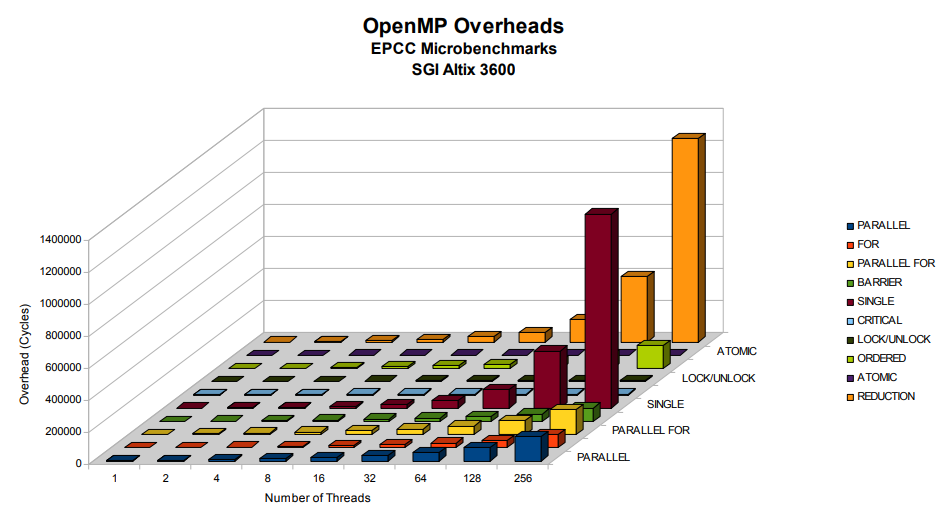
\includegraphics[width=0.8\linewidth]{figures/OpenMP/Overheads_Directives.png}
        \caption{Overheads của một số chỉ thị}
    \end{figure}
\end{frame}

\begin{frame}[fragile]{Một số kỹ thuật tối ưu}
    \begin{itemize}
        \item Giảm tần suất sử dụng barrier với nowait
    \end{itemize}

    \begin{verbatim}
#pragma	omp	parallel	
{	
    #pragma	omp	for
    for(i=0;i<n;i++)	
        ….	
    #pragma	omp	for	nowait
    for(i=0;i<n;i++)	
}	
    \end{verbatim}
\end{frame}

\begin{frame}[fragile]{Một số kỹ thuật tối ưu}
    \begin{verbatim}
#pragma	omp	parallel private(i)	
{	
    #pragma	omp	for	nowait
    for(i=0;i<n;i++)	
        a[i] +=b[i];	
    #pragma	omp	for	nowait
    for(i=0;i<n;i++)	
        c[i] +=d[i];	
    #pragma	omp	barrier	
    #pragma	omp	for	nowait	reducAon(+:sum)	
    for(i=0;i<n;i++)
        sum	+=	a[i]	+	c[i];	
}	
    \end{verbatim}
\end{frame}

\begin{frame}[fragile]{Một số kỹ thuật tối ưu}
    \begin{itemize}
        \item Tránh sử dụng ordered với khối lệnh lớn
        \item Tránh sử dụng critical với khối lệnh lớn
    \end{itemize}
    \begin{verbatim}
    #pragma	omp	parallel shared(a,b) private(c,d)	
    {	
        ...	
        #pragma	omp	critical
        {	
            a += 2*c;	
            c =	d*d; // Nên để biểu thức ra ngoài
        }	
    }	
    \end{verbatim}
\end{frame}

\begin{frame}[fragile]{Một số kỹ thuật tối ưu}
    \begin{itemize}
        \item Parallel regions hãy dài nhất có thể
    \end{itemize}
    \begin{columns}[onlytextwidth]
        \begin{column}{0.5\linewidth}
            \begin{verbatim}
#pragma	omp	parallel		
{	
    #pragma	omp	for	
    for(...) {...}	
}	
opt = opt +	N; // sequential
#pragma	omp	parallel	
{	
    #pragma	omp	for	
    for(...) {...}	
    #pragma	omp	for	
    for(...) {...}	
}    
            \end{verbatim}
        \end{column}
        \begin{column}{0.5\linewidth}
            \begin{verbatim}
#pragma	omp	parallel		
{	
    #pragma	omp	for	
    for(...) {...}	
}
#pragma omp single nowait
opt = opt +	N; // sequential	
#pragma	omp	for	
for(...) {...}	
#pragma	omp	for	
for(...) {...}	
            \end{verbatim}
        \end{column}
    \end{columns}
\end{frame}

\begin{frame}[shrink, fragile]{Một số kỹ thuật tối ưu}
    \begin{itemize}
        \item Một parallel region chứa tất cả các vòng lặp for.
    \end{itemize}
    \begin{columns}[onlytextwidth]
        \begin{column}{0.5\linewidth}
            \begin{verbatim}
for (i = 0; i < n; i++)
    for (j = 0; j < n; j++)
        #pragma omp parallel for \ 
         private(k)
        for (k = 0; k < n; k++) {
            ...
        }
            \end{verbatim}
        \end{column}
        \begin{column}{0.5\linewidth}
            \begin{verbatim}
#pragma omp parallel \
private(i, j, k)
for (i = 0; i < n; i++)
    for (j = 0; j < n; j++)
        #pragma omp for
        for (k = 0; k < n; k++) {
            ...
        }
            \end{verbatim}
        \end{column}
    \end{columns}
\end{frame}

\begin{frame}[fragile]{Một số kỹ thuật tối ưu}
    \begin{itemize}
        \item Tránh chọn chunk size nhỏ
    \end{itemize}
    \begin{columns}[onlytextwidth]
        \begin{column}{0.5\linewidth}
            \begin{figure}[H]
                \centering
                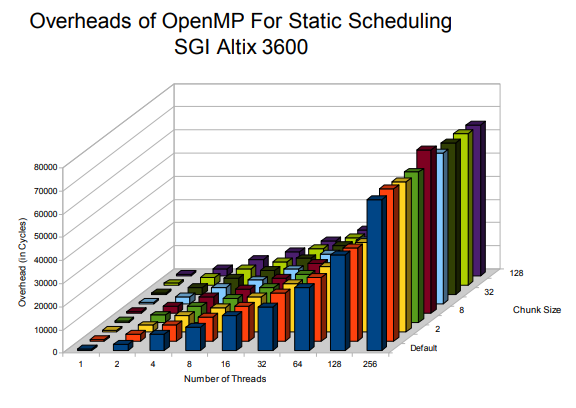
\includegraphics[width=0.9\linewidth]{figures/OpenMP/Overhead_Static_Scheduling_Chunk_Size.png}
            \end{figure}
        \end{column}
        \begin{column}{0.5\linewidth}
            \begin{figure}[H]
                \centering
                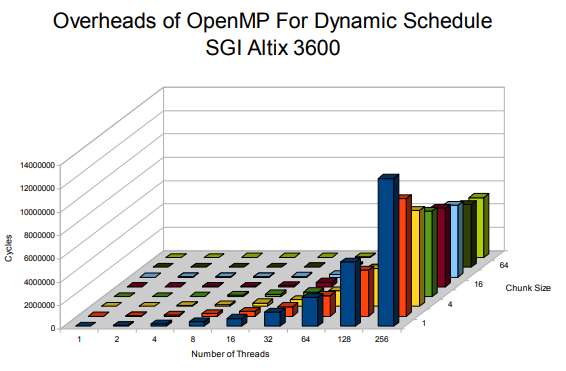
\includegraphics[width=0.9\linewidth]{figures/OpenMP/Overhead_Dynamic_Scheduling_Chunk_Size.png}
            \end{figure}
        \end{column}
    \end{columns}
\end{frame}

\begin{frame}[fragile]{Một số kỹ thuật tối ưu}
    \begin{itemize}
        \item chỉ thị master hiệu quả hơn single nhưng cần thread id 0 sẵn sàng
        \item single hiệu quả hơn nếu thread id 0 không sẵn sàng
        \item single có barrier ngầm, khi không cần thiết nên dùng thêm nowait
    \end{itemize}
\end{frame}

\section{Message Passing Interface}

\subsection{Tổng quan MPI}

\begin{frame}{Tổng quan MPI}
    \begin{itemize}
        \item Là một API tiêu chuẩn cho quá trình truyền thông đẹp, tra cứu thông tin, đăng ký, phân nhóm và tạo mới kiểu dữ liệu thông điệp.
        \item Có thể truyền giao thức theo hai hình thức:
        \begin{itemize}
            \item Truyền điểm - điểm
            \item Truyền quảng bá (một - nhiều, nhiều - một , nhiều - nhiều)
        \end{itemize}
        \item Hỗ trợ lập trình song song mức thấp
        \item Được hỗ trợ trên Fortran 77 và C, MPI2 được hỗ trợ trên C++/Fortran90
        \item Một API rất lớn (128 hàm), MPI-2 có thêm 152 hàm. Đa số người dùng chỉ dùng một phần.
        \item Hướng hiệu năng
    \end{itemize}
\end{frame}

\begin{frame}[shrink]{Lịch sử MPI}
    \begin{itemize}
        \item Nhiều thư viện truyền thông đẹp đã được tạo ra trong quá khứ:
        \begin{itemize}
            \item TCGMSG, P4, PARMACS, EXPRESS, NX, MPL, PVM
        \end{itemize}
        \item 1992-1994 diễn đàn về truyền thông điệp định nghĩa một tiêu chuẩn mới cho truyền thông điệp (ban đầu đặt là MPPs)
        \item Quá trình phát triển của tiêu chuẩn:
        \begin{itemize}
            \item 1994: MPI 1.0: các giao tiếp cơ bản, Fortran77 và C
            \item 1995: MPI 1.1: sửa lỗi bản trước
            \item 1997: MPI 2.0: Giao tiếp 1 phía, I/O, khởi tạo tiến trình, Fortran 99 và C, giải thích các hàm rõ hơn. Bao gồm MPI 1.2.
            \item 2008: MPI 1.3, 2.1: kết hợp 1.3 và 2.0
            \item 2009: MPI 2.2: sửa lỗi và giải thích các hàm
            \item MPI 3.0 đang trong quá trình chuẩn hóa và hoàn thiện
        \end{itemize}
    \end{itemize}
\end{frame}

\begin{frame}{Bản đồ phát triển}
    \begin{figure}[H]
        \centering
        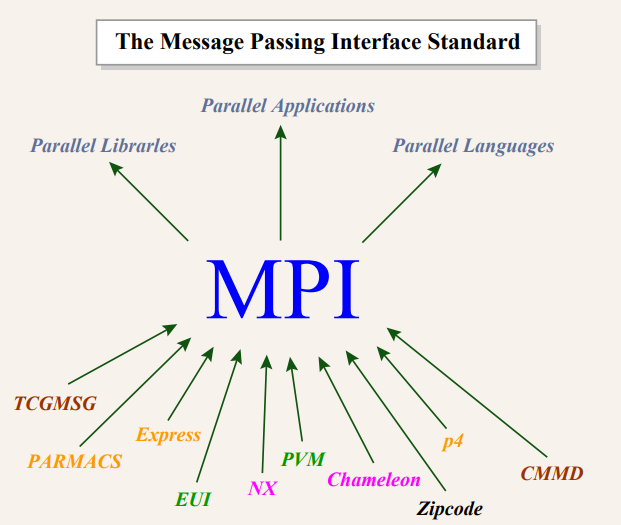
\includegraphics[width=0.75\linewidth]{figures/MPI/MPI_Genealogy.png}
        \caption{Quá trình phát triển của MPI}
    \end{figure}
\end{frame}

\begin{frame}[shrink]{MPI cơ bản}
    \begin{itemize}
        \item Góc nhìn logic của nền tảng truyền thông điệp:
        \begin{itemize}
            \item p tiến trình
            \item Mỗi tiền trình có một không gian bộ nhớ riêng
        \end{itemize}
        \item Tất cả dữ liệu phải cần được phân chia rõ ràng
        \begin{itemize}
            \item Tiến trình cần truyền dữ liệu
            \item Tiến trình cần nhận dữ liệu
        \end{itemize}
        \item Thường sử dụng mô thức lập trình (SIMD)
        \item Ưu điểm:
        \begin{itemize}
            \item Mô hình hiệu năng đơn giản: chi phí ngầm dễ tính
            \item Hiệu năng và tính linh hoạt cao
        \end{itemize}
        \item Nhược điểm: Mô hình truyền thông điệp hai phía làm chương trình phức tạp
    \end{itemize}
\end{frame}

\begin{frame}{MPI cơ bản}
    \begin{itemize}
        \item Hướng dẫn cài đặt MPI trên Windows: \url{https://www.youtube.com/watch?v=T_BVqSya1Is}
        \item Setup cluster MPI: \url{https://mpitutorial.com/tutorials/running-an-mpi-cluster-within-a-lan/}
    \end{itemize}
\end{frame}

\begin{frame}{MPI cơ bản}
    \begin{itemize}
        \item File tiêu đề mpi.h cho C/C++ và mpif.h cho Fortran
        \item Tất cả các hàm đều trả về giá trị lỗi
        \item Trong C/C++, các đối số được truyền vào dạng con trỏ
        \item Luôn luôn bắt đầu với MPI\_Init() và kết thúc với MPI\_Finalize() (hoặc MPI\_Abort()).
        Hai hàm trên đều cần được gọi bởi tất cả các tiến trình
        \item Tất cả các hàm, kiểu dữ liệu, hằng số đều có tiền tố là "MPI\_"
        \item Một chương trình MPI có thể chỉ cần sử dụng 6 hàm thư viện
    \end{itemize}
\end{frame}

\begin{frame}{MPI cơ bản}
    \begin{figure}[H]
        \centering
        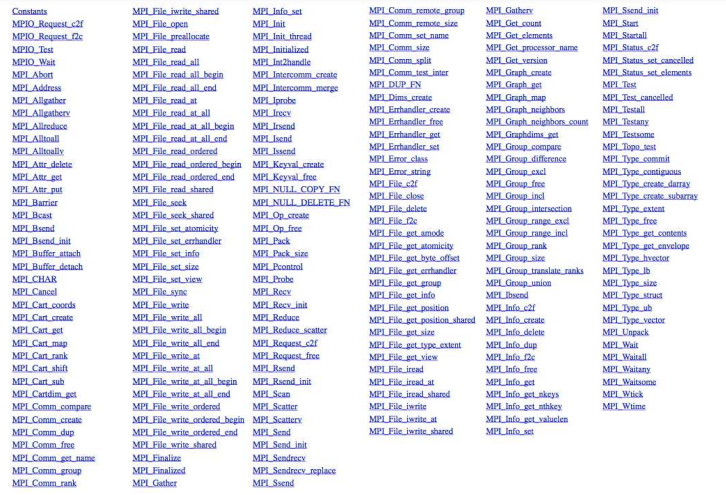
\includegraphics[height=0.85\textheight]{figures/MPI/MPI_Full_Routines.png}
    \end{figure}
\end{frame}

\begin{frame}{Một số hàm thông dụng}
    \begin{table}[H]
        \centering
        \begin{tabular}{|l|l|}
            \hline
            MPI\_Init & Khởi tạo môi trường MPI \\
            \hline
            MPI\_Finalize & Ngắt môi trường MPI \\
            \hline
            MPI\_Comm\_size & Xác định số tiến trình \\
            \hline
            MPI\_Comm\_rank & Xác định id của tiến trình gọi hàm trong nhóm \\
            \hline
            MPI\_Send & Truyền thông điệp \\
            \hline
            MPI\_Recv & Nhận thông điệp \\
            \hline
        \end{tabular}
    \end{table}
    
\end{frame}

\begin{frame}{Khởi tạo và ngắt môi trường MPI}
    \begin{itemize}
        \item int MPI\_Init(int *argc, char ***argv) 
        \begin{itemize}
            \item Câu lệnh được gọi trước các hàm khác của MPI
            \item Khởi tạo môi trường MPI
        \end{itemize}
        \item int MPI\_Finalize()
        \begin{itemize}
            \item Được gọi khi kết thúc tính toán
            \item Ngắt môi trường MPI
        \end{itemize}
        \item Mã trả về:
        \begin{itemize}
            \item MPI\_SUCCESS
            \item MPI\_ERROR
        \end{itemize}
    \end{itemize}
\end{frame}

\begin{frame}{Bộ giao tiếp}
    \begin{itemize}
        \item MPI\_Comm: nhóm các tiến trình có thể giao tiếp với nhau
        \item Được truyền vào là đối số của một hàm truyền thông điệp
        \item Một tiến trình có thể thuộc về nhiều nhóm khác nhau
        \item MPI\_COMM\_WORLD: bộ giao tiếp toàn cục bao gồm tất cả các tiến trình
    \end{itemize}
    \begin{figure}[H]
        \centering
        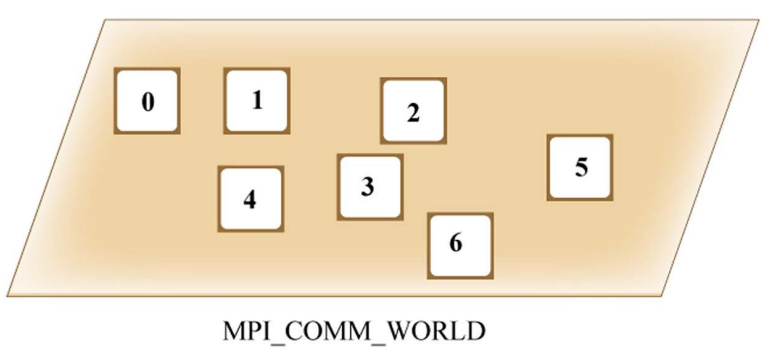
\includegraphics[height=0.4\textheight]{figures/MPI/MPI_COMM_WORLD.png}
    \end{figure}
\end{frame}

\begin{frame}{Truy vấn bộ giao tiếp}
    \begin{itemize}
        \item int MPI\_Comm\_size(MPI\_Comm comm, int *size) : xác định số tiến trình
        \item int MPI\_Comm\_rank(MPI\_Comm comm, int *rank) : xác định chỉ số của tiến tình gọi hàm ($0 \leq rank <$ số tiến trình trong nhóm)
    \end{itemize}
    \begin{figure}[H]
        \centering
        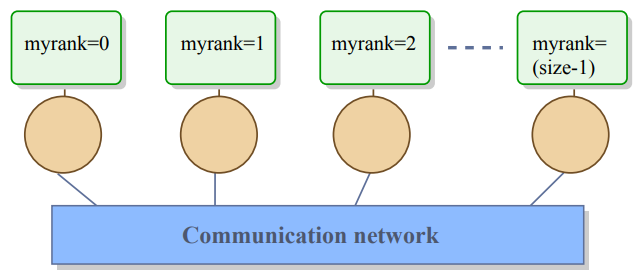
\includegraphics[height=0.4\textheight]{figures/MPI/Rank.png}
    \end{figure}
\end{frame}

\begin{frame}{Ngắt môi trường MPI}
    \begin{itemize}
        \item int MPI\_Finalize(): Ngắt kết nối môi trường MPI
        \item int MPI\_Abort(MPI\_Comm comm, int errorcode): Nếu một tiến trình bắt được một lỗi và không xử lý được
    \end{itemize}
\end{frame}

\begin{frame}[fragile]{Chương trình MPI Hello World}
    \begin{verbatim}
#include<stdio.h>
#include<mpi.h>
int main(int argc, char** argv) {
    int size, rank;
    MPI_Init(&argc, &argv);
    MPI_Comm_size(MPI_COMM_WORLD, &size);
    MPI_Comm_rank(MPI_COMM_WORLD, &rank);
    printf("From process %d out of %d processes", rank, size);
    MPI_Finalize();
    return 0;
}
    \end{verbatim}
\end{frame}

\begin{frame}{Truyền thông}
    \begin{itemize}
        \item Giao tiếp truyền thông điệp có thể giữa hai tiến trình hoặc giữa một nhóm các tiến trình
        \item Truyền thông thường là truyền mảng dữ liệu tổ chức theo kiểu dữ liệu MPI:
        \begin{itemize}
            \item Kiểu dữ liệu được định nghĩa là ánh xạ tớ kiểu dữ liệu của ngôn ngữ lập trình sử dụng MPI.
            \item Kiểu dữ liệu người do người dùng định nghĩa, các cấu trúc hoặc các kiểu dữ liệu khác
            \item Kiểu dứ liệu do người dùng định nghĩa sẽ được MPI tối ưu
        \end{itemize}
    \end{itemize}
\end{frame}

\begin{frame}{Các kiểu dữ liệu nguyên thủy của MPI}
    \begin{table}[H]
        \centering
        \begin{tabular}{ll}
            \hline
            Kiểu dữ liệu của MPI & Kiểu dữ liệu của C \\
            \hline
            MPI\_CHAR & signed char \\
            MPI\_SHORT & signed short int \\
            MPI\_INT & signed int \\
            MPI\_LONG & signed long int \\
            MPI\_UNSIGNED\_CHAR & unsigned char \\
            MPI\_UNSIGNED\_SHORT & unsigned short int \\
            MPI\_UNSIGNED & unsigned int \\
            MPI\_UNSIGNED\_LONG & unsigned long int \\
            MPI\_FLOAT & float \\
            MPI\_DOUBLE & double \\
            MPI\_LONG\_DOUBLE & long double \\
            MPI\_BYTE & 8 bits \\
            MPI\_PACKED & dãy bytes được đóng gói \\
            \hline
        \end{tabular}
    \end{table}
\end{frame}

\begin{frame}{Thông điệp}
    Một thông điệp bao gồm các trường thông tin:
    \begin{itemize}
        \item Địa chỉ người gửi
        \item Nơi lưu trữ thông điệp
        \item Kiểu dữ liệu thông điệp
        \item Kích thước thông điệp
        \item Thẻ thông điệp
        \item Địa chỉ người nhận 
        \item Nơi lưu trữ nhận thông điệp
        \item Kiểu dữ liệu phù hợp nơi nhận 
        \item Thẻ thông điệp khớp với bên gửi
    \end{itemize}
\end{frame}

\subsection{Truyền thông điệp điểm - điểm trong MPI}

\begin{frame}{Truyền thông điệp điểm - điểm}
    \begin{itemize}
        \item Giao tiếp blocking: Chờ đến khi truyền thông điệp hoàn thành
        \item Giao tiếp non-blocking: Trả về không cần đợi khi truyền thông điệp hoàn thành
        \item Các hình thức gửi:
        \begin{itemize}
            \item Đồng bộ: thông điệp chỉ được gửi khi biết chắc chắn có người đã sẵn sàng đợi nhận ở phía bên kia (fax).
            \item Bộ đệm: tin nhắn được gửi đi nếu người bên kia đang đợi hoặc nếu không sẽ được lưu vào một bộ đệm tạm thời cho đến khi lấy thông điệp khỏi bộ đệm.
            \item Kiểu sẵn sàng: giống như đồng bộ nhưng không có xác nhận từ bên nhận.
        \end{itemize}
    \end{itemize}
\end{frame}

\begin{frame}{Truyền thông điệp có blocking của MPI}
    \begin{itemize}
        \item int MPI\_Send(void *buf, int count, MPI\_Datatype datatype,
                            int dest, int tag, MPI\_Comm comm);
        \begin{itemize}
            \item buf là địa chỉ bắt đầu chứa thông điệp cần được truyền
            \item count là số phần tử của thông điệp
            \item datatype là kiểu dữ liệu của thông điệp
            \item dest là rank của tiến trình nhận thông điệp
            \item tag là một số định danh của thông điệp, thống nhất giữa bên gửi và bên nhận
            \item comm là bộ giao tiếp
        \end{itemize}
        \item Ví dụ: MPI\_Send(A, ns, MPI\_INT, 1, 0, MPI\_COMM\_WORLD): 
        Truyền ns phần tử kiểu int từ địa chỉ A sang tiến trình 1 với tag là 0.
    \end{itemize}
\end{frame}

\begin{frame}{Truyền thông điệp có blocking của MPI}
    \begin{itemize}
        \item MPI\_Ssend: Gửi đồng Bộ
        \begin{itemize}
            \item Người gửi thông báo người nhận, người nhận xác nhận sẵn sàng và người gửi gửi thông điệp.
        \end{itemize}
        \item MPI\_Bsend: Gửi bộ đệm
        \begin{itemize}
            \item Người gửi đưa dữ liệu và một bộ đệm và trả về ngay lập tức khi quá trình sao chép dữ liệu vào bộ đệm bên người gửi hoàn thành
        \end{itemize}
        \item MPI\_Rsend: Gửi sẵn sàng
        \begin{itemize}
            \item Người nhận được thông báo và dữ liệu được gửi ngay
        \end{itemize}
    \end{itemize}
\end{frame}

\begin{frame}{Một số lưu ý khi gửi thông điệp blocking}
    \begin{itemize}
        \item Đối với dữ liệu nhỏ, có thể dùng bộ đệm, đồng bộ phù hợp với dữ liệu lớn hơn
        \item MPI\_Ssend có thể gây ra deadlock
    \end{itemize}
\end{frame}

\begin{frame}{Hiệu năng của truyền thông điệp blocking}
    \begin{itemize}
        \item Truyền đồng bộ  cho tốc độ truyền dữ liệu cao nhất, nhưng chi phí khở tạo lại rất cao (độ trễ) và nguy cơ xảy ra deadlock.
        \item Truyền bộ đệm cho độ trễ thấp nhất nhưng:
        \begin{itemize}
            \item Quản lý bộ đệm phức tạp
            \item Vấn đề về băng thông do chi phí sao chép
        \end{itemize}
        \item Gửi sẵn sàng có vẻ là tốt nhất nhưng cũng rất dễ gây khó khăn trong lập trình nên cũng tránh sử dụng
        \item Truyền theo tiêu chuẩn cần phải được tối ưu cẩn thận. Với thông điệp kích thước lớn gần như chắc chắn xảy ra deadlock
    \end{itemize}
    
\end{frame}

\begin{frame}{Nhận thông điệp có blocking của MPI}
    \begin{itemize}
        \item int MPI\_Recv(void *buf, int count, MPI\_Datatype datatype,
                            int source, int tag, MPI\_Comm comm,
                            MPI\_Status *status)
        \begin{itemize}
            \item buf là địa chỉ bắt đầu chứa thông điệp nhận được
            \item count là số phần tử của thông điệp
            \item datatype là kiểu dữ liệu của thông điệp
            \item source là rank của tiến trình gửi thông điệp
            \item tag là một số định danh của thông điệp, thống nhất giữa bên gửi và bên nhận
            \item comm là bộ giao tiếp
            \item status là địa chỉ biến nhận trạng thái
        \end{itemize}
        \item Ví dụ: MPI\_Recv(B, ns, MPI\_INT, 0, 1, MPI\_COMM\_WORLD, \&status);
    \end{itemize}
\end{frame}

\begin{frame}{Một số vấn đề về nhận thông điệp có blocking của MPI}
    \begin{itemize}
        \item Bộ đệm có thể có kích thước không đúng hoặc kiểu dữ liệu được cấp phát không phù hợp với thông điệp nhận được thì bộ đệm có thể mất dữ liệu hoặc có dữ liệu nhiễu.
        \item Các thông tin như source, tag được lưu trong biến MPI\_Status
        \item Biến errorcode có thể dùng để phục vụ cho quá trình debug
        \item Nếu bất kỳ tiến trình nào trong nhóm có thể là source thì dùng thẻ MPI\_ANY\_source
        \item Nếu bất kỳ tag nào cũng được chấp nhận có thể dùng thẻ MPI\_ANY\_TAG
        \item Độ dài thông điệp $\leq$ độ dài bộ đệm đã đặt trước
        \item Thứ tự nhận và gửi bản tin là quan trọng
    \end{itemize}
\end{frame}

\begin{frame}[fragile]{Một số biến trạng thái bên nhận}
    \begin{itemize}
        \item MPI\_Status
        \begin{itemize}
            \item Lưu thông tin về quá trình của hàm nhận MPI\_Recv
            \item Là một biến cấu trúc:
            \begin{verbatim}
typedef struct MPI_Status {
    int MPI_SOURCE;
    int MPI_TAG;
    int MPI_ERROR; };
            \end{verbatim}
        \end{itemize}
        \item int MPI\_Get\_count(MPI\_Status *status, MPI\_Datatype datatype, int *count) 
        \begin{itemize}
            \item Trả về số phần tử dữ liệu đã nhận được 
        \end{itemize}
    \end{itemize}
\end{frame}

\begin{frame}[shrink, fragile]{Deadlock với MPI\_Send / MPI\_Recv}
    \begin{verbatim}
int a[10], b[10], rank;
MPI_Status s1, s2;
...
MPI_Comm_rank(MPI_COMM_WORLD, &rank);
if (rank == 0) {
    MPI_Send(a, 10, MPI_INT, 1, 1, MPI_COMM_WORLD);
    MPI_Send(b, 10, MPI_INT, 1, 2, MPI_COMM_WORLD);
}
else if (rank == 1) {
    MPI_Recv(b, 10, MPI_INT, 0, 2, MPI_COMM_WORLD, &s1);
    MPI_Recv(a, 10, MPI_INT, 0, 1, MPI_COMM_WORLD, &s2);
}
...
    \end{verbatim}

    \begin{itemize}
        \item Deadlock xảy ra do tiến trình 0 gửi mảng a trước khi gửi mảng b, nhưng tiến trình 1 lại đợi nhận mảng b trước khi gửi mảng a
    \end{itemize}
\end{frame}

\begin{frame}[fragile]{Deadlock khi truyền thông điệp theo vòng tròn khép kín}
    \begin{verbatim}
int a[10], b[10], size, rank;
MPI_Status status;
...
MPI_Comm_size(MPI_COMM_WORLD, &size);
MPI_Comm_rank(MPI_COMM_WORLD, &rank);
MPI_Send(a, 10, MPI_INT, (rank+1)%size, 1,
 MPI_COMM_WORLD);
MPI_Recv(b, 10, MPI_INT, (rank-1+size)%size, 1,
    MPI_COMM_WORLD, &status);
... 
    \end{verbatim}
    Mỗi tiến trình gửi thông điệp sang tiến trình kề bên phải và tiến trình cuối cùng gửi thông điệp cho tiến trình đầu tiên tạo thành một vòng tròn khép kín
\end{frame}

\begin{frame}[shrink, fragile]{Khắc phục tình trạng deadlock}
    \begin{verbatim}
int a[10], b[10], size, rank;
MPI_Status status;
...
MPI_Comm_size(MPI_COMM_WORLD, &size);
MPI_Comm_rank(MPI_COMM_WORLD, &rank);
if (rank%2 == 1) { // tiến trình lẻ gửi trước, nhận sau
    MPI_Send(a, 10, MPI_INT, (rank+1)%size, 1, MPI_COMM_WORLD);
    MPI_Recv(b, 10, MPI_INT, (rank-1+size)%size, 1,
    MPI_COMM_WORLD, &status);
}
else { // tiến trình chẵn nhận trước, gửi sau
    MPI_Recv(b, 10, MPI_INT, (rank-1+size)%size, 1,
             MPI_COMM_WORLD, &status);
     MPI_Send(a, 10, MPI_INT, (rank+1)%size, 1,
             MPI_COMM_WORLD);
    }
...     
    \end{verbatim}
\end{frame}

\begin{frame}{Truyền thông điệp hai chiều}
    \begin{itemize}
        \item Trong trường hợp hai tiến trình trao đổi thông điệp đồng thời hoặc một tiến trình đang gửi thông điệp khi đang nhận từ một tiến trình khác
        \begin{itemize}
            \item int MPI\_Sendrecv(void *sendbuf, int sendcount,
                                    MPI\_Datatype senddatatype, int dest, int sendtag,
                                    void *recvbuf, int recvcount, MPI\_Datatype recvdatatype,
                                    int source, int recvtag, MPI\_Comm comm,
                                    MPI\_Status *status)
            \item int MPI\_Sendrecv\_replace(void *buf, int count,
                                             MPI\_Datatype datatype, int dest, int sendtag,
                                             int source, int recvtag, MPI\_Comm comm,
                                             MPI\_Status *status)
        \end{itemize}
        \item MPI\_Sendrecv rất hữu dụng khi truyền tin lần lượt trong một vòng tròn khép kín và tránh được deadlock mà không cần dùng phương pháp chẵn, lẻ.
        MPI sẽ tự động xử ý vấn đề này
    \end{itemize}
\end{frame}

\begin{frame}{Truyền thông điệp non-blocking trong MPI}
    \begin{itemize}
        \item Các hàm gửi và truyền thông điệp non-blocking trả về trước khi quá trình giao tiếp hoàn tất 
        \begin{itemize}
            \item int MPI\_Isend(void *buf, int count, MPI\_Datatype datatype,
                                int dest, int tag, MPI\_Comm comm,
                                MPI\_Request *request) 
            \item int MPI\_Irecv(void *buf, int count, MPI\_Datatype datatype,
                                   int source, int tag, MPI\_Comm comm,
                                   MPI\_Request *request)
        \end{itemize}
    \end{itemize}
\end{frame}

\begin{frame}{Truyền thông điệp non-blocking trong MPI}
    \begin{itemize}
        \item MPI\_Test: Kiểm tra xem một quá trình giao tiếp đã kết thúc chưa
        \begin{itemize}
            \item int MPI\_Test(MPI\_Request *request, int *flag,
                                MPI\_Status *status) 
        \end{itemize}
        \item MPI\_Waitany: chờ đến khi ít nhất một trong các truyền thông trong tập hoàn thành
        \begin{itemize}
            \item int MPI\_Waitany(int req\_cnt, MPI\_Request *req\_array,
                                   int *req\_index, MPI\_Status *status) 
        \end{itemize}
        \item MPI\_Wait: chờ đến khi một truyền thông cụ thể hoàn Tất
        \begin{itemize}
            \item int MPI\_Wait(MPI\_Request *request, MPI\_Status *status)
        \end{itemize}
    \end{itemize}
\end{frame}

\begin{frame}[shrink, fragile]{Truyền thông điệp non-blocking trong MPI}
    \begin{verbatim}
int rank, size;
int data_send, data_recv;
MPI_Request request;
MPI_Status status;
MPI_Init(&argc, &argv);
MPI_Comm_rank(MPI_COMM_WORLD, &rank);
MPI_Comm_size(MPI_COMM_WORLD, &size);
data_send = rank;
// Send data in a ring from process 0 to process (size - 1)
MPI_Isend(&data_send, 1, MPI_INT, 
(rank + 1) % size, 0, MPI_COMM_WORLD, &request);
MPI_Recv(&data_recv, 1, MPI_INT, 
(rank + size - 1) % size, 0, MPI_COMM_WORLD, &status);
MPI_Wait(&request, &status); 
printf("Process %d received data: %d\n", rank, data_recv);
MPI_Finalize();
    \end{verbatim}
\end{frame}

\subsection{Truyền thông điệp quảng bá trong MPI}

\begin{frame}{Truyền thông điệp quảng bá}
    \begin{itemize}
        \item Truyền thông quảng bá là truyền thông giữa một nhóm các tiến trình
        \item Tất cả các bộ đệm bên nhận có cùng kích thước và khác với bộ đệm nhận 
        \item Việc truyền thông điệp có thể là một - tất cả, tất cả - một, tất cả - tất cả.
        \item Nhiều hàm có biến thể dạng vector có tên hàm dạng MPI\_xxxxv
    \end{itemize}
\end{frame}

\begin{frame}{Hàm đồng bộ}
    \begin{itemize}
        \item MPI\_Barrier(MPI\_Comm comm)
        \item Đợi tất cả các tiến trình tiến tới barrier
        \item Chi phí lớn khi số tiến trình nhiều, chỉ sử dụng khi thực sự cần
    \end{itemize}
\end{frame}

\begin{frame}{Truyền thông điệp một - tất cả}
    \begin{itemize}
        \item int MPI\_Bcast(void *buf, int count,
                             MPI\_Datatype datatype, int source,
                             MPI\_Comm comm)
    \end{itemize}

    \begin{figure}[H]
        \centering
        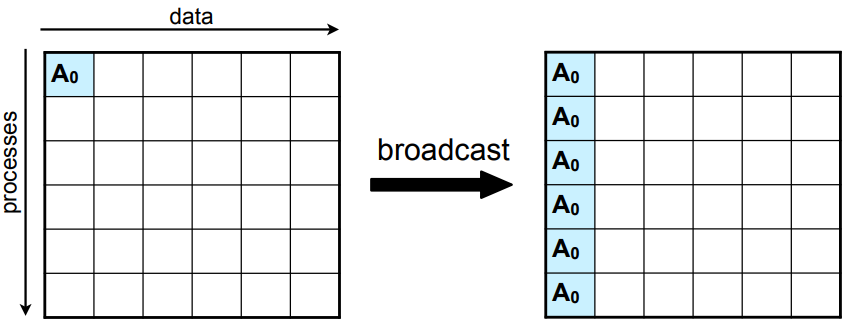
\includegraphics[height=0.5\textheight]{figures/MPI/Bcast.png}
        \caption{Minh họa hàm Bcast}
    \end{figure}
\end{frame}

\begin{frame}{Hàm reduce tất cả - một}
    \begin{itemize}
        \item int MPI\_Reduce(void *sendbuf, void *recvbuf,
                             int count, MPI\_Datatype datatype,
                             MPI\_Op op, int target, MPI\_Comm comm)
        \item Ví dụ MPI\_Op: tổng, tích, min, max
    \end{itemize}

    \begin{figure}[H]
        \centering
        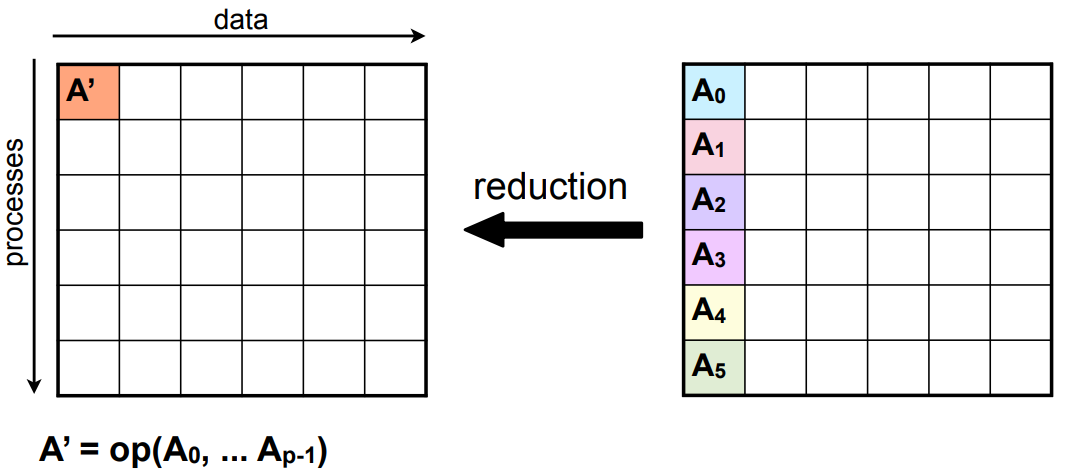
\includegraphics[height=0.5\textheight]{figures/MPI/Reduction_All_To_One.png}
    \end{figure}
\end{frame}

\begin{frame}{Hàm reduce tất cả - một}
    \begin{table}[H]
        \centering
        \resizebox{\columnwidth}{!}{
            \begin{tabular}{lll}
                \hline
                Toán tử & Ý nghĩa & Kiểu dữ liệu \\
                \hline
                MPI\_MAX & Maximum & Các điểm số nguyên và số thực \\
                MPI\_MIN & Minimum & Các điểm số nguyên và số thực \\
                MPI\_SUM & Tổng & Các điểm số nguyên và số thực \\
                MPI\_PROD & Tích & Các điểm số nguyên và số thực \\
                MPI\_LAND & Logical AND & Số nguyên \\
                MPI\_BAND & Bit-wise AND & Số nguyên và byte \\
                MPI\_LOR & Logical OR & Số nguyên \\
                MPI\_BOR & Bit-wise OR & Số nguyên và byte \\
                MPI\_LXOR & Logical XOR & Số nguyên \\
                MPI\_BXOR & Bit-wise XOR & Số nguyên và byte \\
                MPI\_MAXLOC & Giá trị lớn nhất và vị trí tương ứng & Các cặp dữ liệu \\
                MPI\_MINLOC & Giá trị nhỏ nhất và vị trí tương ứng & Các cặp dữ liệu \\
                \hline
            \end{tabular}
        }
    \end{table}
\end{frame}

\begin{frame}{Toán tử MPI\_MINLOC và MPI\_MAXLOC}
    \begin{itemize}
        \item MPI\_MAXLOC:
        \begin{itemize}
            \item Kết hợp từng cặp dữ liệu ($v_i, l_i$)
            \item Trả về cặp ($v, l$) sao cho:
            \begin{itemize}
                \item v là giá trị lớn nhất trong các điểm $v_i$
                \item l là vị trí tương ứng của v
            \end{itemize}
        \end{itemize}
        \item MPI\_MINLOC tương tự
    \end{itemize}
\end{frame}

\begin{frame}{Kiểu dữ liệu cho MPI\_MINLOC và MPI\_MAXLOC}
    \begin{table}[H]
        \centering
        \begin{tabular}{ll}
            \hline
            Kiểu dữ liệu MPI & Kiểu dữ liệu C \\
            \hline
            MPI\_2INT & 2 số nguyên \\
            MPI\_SHORT\_INT & short và int \\
            MPI\_LONG\_INT & long và int \\
            MPI\_LONG\_DOUBLE\_INT & long double và int \\
            MPI\_FLOAT\_INT & float và int \\
            MPI\_DOUBLE\_INT & double và int \\
        \end{tabular}
    \end{table}
\end{frame}

\begin{frame}{Toán tử nhị phân do người dùng định nghĩa}
    \begin{itemize}
        \item MPI cho phép người dùng định nghĩa toán tử nhị phân cho các hàm reduction
        \item int MPI\_Op\_create(MPI\_User\_function *function, int commute,
                            MPI\_Op *op)
        \item Nếu commute là khác 0, toán tử là giao hoán. Nếu không toán tử chỉ thỏa mãn tính chất kết hợp
        \item Hàm (non MPI) cần có dạng:
        \begin{itemize}
            \item typedef void MPI\_User\_function (void *invec, void *inoutvec,
                                                    int *len, MPI\_Datatype *type) 
        \end{itemize}
    \end{itemize}
\end{frame}

\begin{frame}{Reduction tất cả - tất cả và tổng tiền tố}
    \begin{itemize}
        \item Reduction tất cả - tất cả: mỗi tiến trình nhận được một bản sao của kết quả
        \begin{itemize}
            \item int MPI\_Allreduce(void *sendbuf, void *recvbuf,
                                    int count, MPI\_Datatype datatype,
                                    MPI\_Op op, MPI\_Comm comm)

           \item Tương đương với hai hàm MPI\_Reduce + MPI\_Bcast
        \end{itemize}
        \item Các phép toán tiền tốc
        \begin{itemize}
            \item inclusive scan: kết quả ở tiến trình i = op($v_0, ... v_i$) 
            \item int MPI\_Scan(void *sendbuf, void *recvbuf, int count,
                               MPI\_Datatype datatype, MPI\_Op op,
                               MPI\_Comm comm)
            \item exclusive scan: kết quả ở tiến trình i = op($v_0, ... v_{i-1}$) 
            \item int MPI\_Exscan(void *sendbuf, void *recvbuf, int count,
                                  MPI\_Datatype datatype, MPI\_Op op,
                                  MPI\_Comm comm)
           
        \end{itemize}
    \end{itemize}
\end{frame}

\begin{frame}{MPI\_Scatter}
    \begin{itemize}
        \item Chia dữ liệu thành p blocks và truyền p-1 blocks từ tiến trình 0 sang các tiến trình còn lại (mỗi tiến trình 1 block)
        \item int MPI\_Scatter(void *sendbuf, int sendcount,
                               MPI\_Datatype senddatatype, void *recvbuf,
                               int recvcount, MPI\_Datatype recvdatatype,
                               int source, MPI\_Comm comm) 
        \item sendcount là số phần tử được gửi tới từng tiến trình (số phần tử trong 1 block)
    \end{itemize}
\end{frame}

\begin{frame}{MPI\_Gather}
    \begin{itemize}
        \item Tập hợp dữ liệu về một tiến trình
        \item int MPI\_Gather(void *sendbuf, int sendcount,
                             MPI\_Datatype senddatatype, void *recvbuf,
                             int recvcount, MPI\_Datatype recvdatatype,
                             int target, MPI\_Comm comm)
        \item sendcount là số phần tử được gửi từ các tiến trình
    \end{itemize}
\end{frame}

\begin{frame}{MPI\_Scatter/MPI\_Gather}
    \begin{figure}[H]
        \centering
        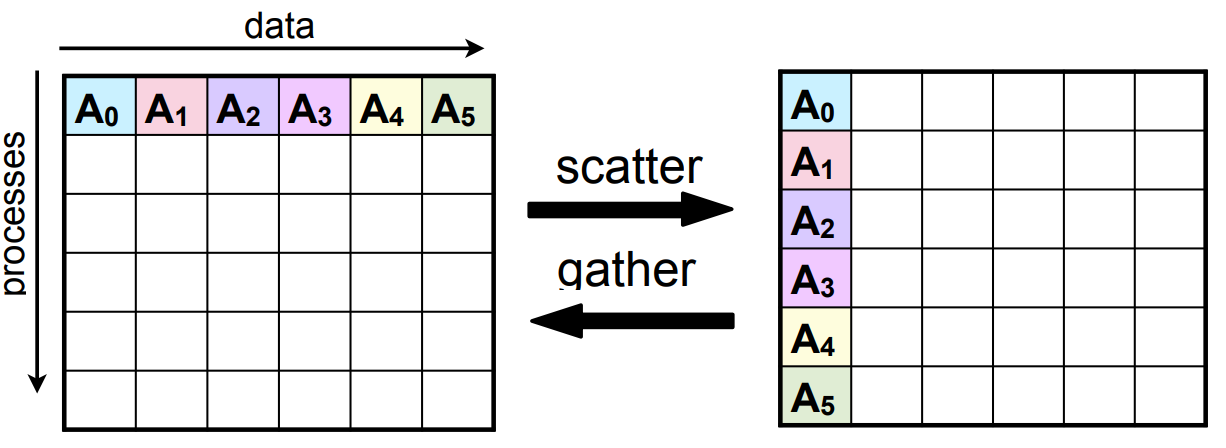
\includegraphics[width=0.8\textwidth]{figures/MPI/Scatter_Gather.png}
        \caption{Minh họa hai hàm MPI\_Scatter/MPI\_Gather}
    \end{figure}
\end{frame}

\begin{frame}{Hàm MPI\_Allgather}
    \begin{itemize}
        \item Giống như hàm MPI\_Gather nhưng không truyền tới một tiến trình duy nhất mà gửi các bản sao kết quả tới tất cả các tiến trình
        \item int MPI\_AllGather(void *sendbuf, int sendcount,
                                MPI\_Datatype senddatatype, void *recvbuf,
                                int recvcount, MPI\_Datatype recvdatatype,
                                MPI\_Comm comm)
    \end{itemize}
    \begin{figure}[H]
        \centering
        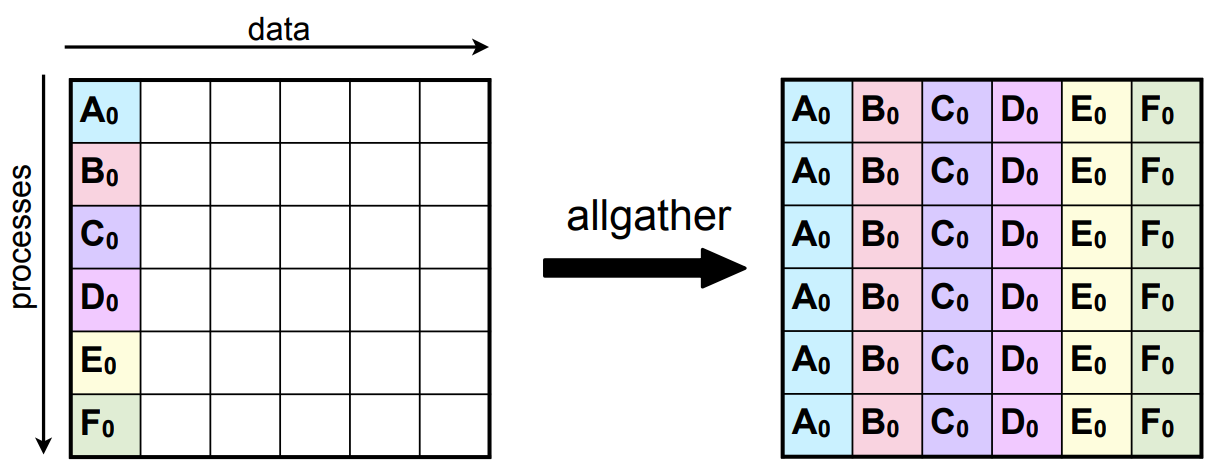
\includegraphics[height=0.45\textheight]{figures/MPI/Allgather.png}
        \caption{Minh họa hàm MPI\_Allgather}
    \end{figure}
\end{frame}

\begin{frame}{Truyền thông tất cả - tất cả}
    \begin{itemize}
        \item Mỗi tiến trình có một tập các block dữ liệu
        \item Mỗi tiến trình truyền kiểu scatter đến các tiến trihf còn lại
        \item Kết quả tương đương với chuyển vị ma trận
        \item int MPI\_Alltoall(void *sendbuf, int sendcount,
                                MPI\_Datatype senddatatype, void *recvbuf,
                                int recvcount, MPI\_Datatype recvdatatype,
                                MPI\_Comm comm) 
    \end{itemize}

    \begin{figure}[H]
        \centering
        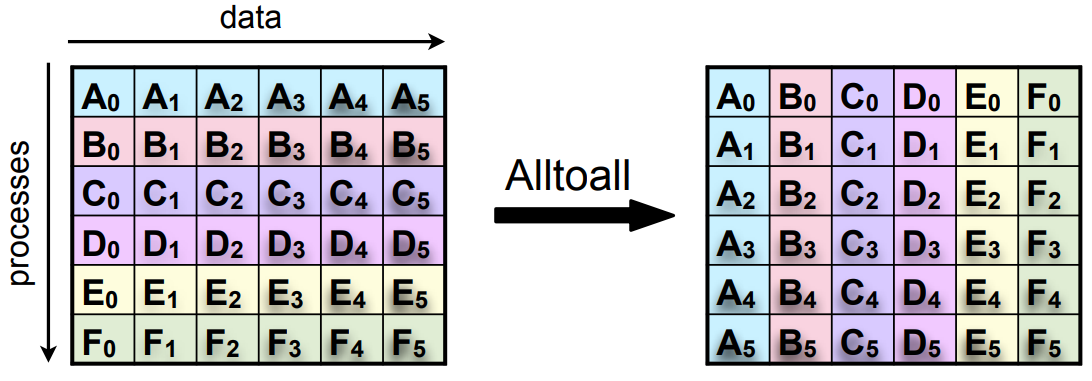
\includegraphics[height=0.35\textheight]{figures/MPI/Alltoall.png}
        \caption{Minh họa hàm MPI\_Alltoall}
    \end{figure}
\end{frame}

\subsection{Phân nhóm các tiến trình}

\begin{frame}{Tách bộ giao tiếp}
    \begin{itemize}
        \item Hữu ích khi phân hoạch bộ giao tiếp cho các tập con tiến trình
        \item MPI cũng cung cấp cơ chế giúp phân hoạch thành các nhóm tiến trình
        \item int MPI\_Comm\_split(MPI\_Comm comm, int color, int key,
                                   MPI\_Comm *newcomm)
        \begin{itemize}
            \item Phân nhóm dữ liệu bằng màu sắc
            \item Sắp xếp các nhóm bởi key
        \end{itemize}
    \end{itemize}
\end{frame}

\begin{frame}{Tách bộ giao tiếp}
    \begin{figure}[H]
        \centering
        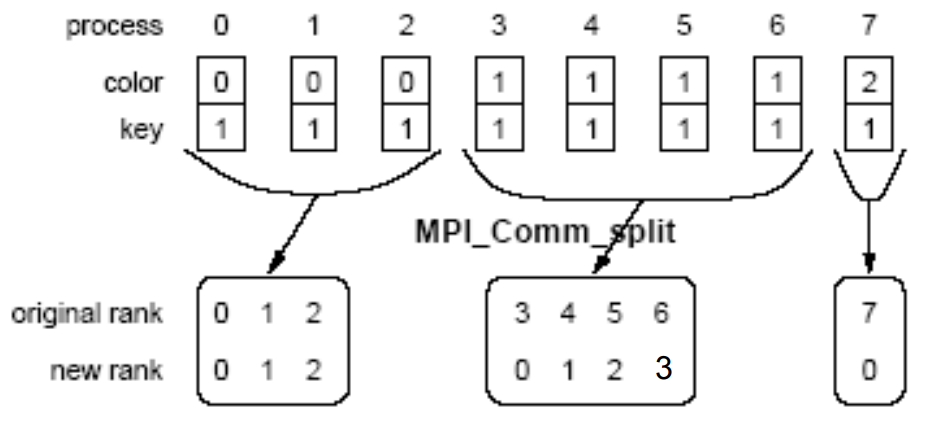
\includegraphics[width=0.7\linewidth]{figures/MPI/Split_Communicator.png}
        \caption{Sử dụng MPI\_Comm\_split để tách nhóm các tiến trình trong một bộ giao tiếp thành các nhóm nhỏ}
    \end{figure}
\end{frame}

\begin{frame}{Topology của các tiến trình}
    \begin{itemize}
        \item Các tiến trình trong MPI\_COMM\_WORLD có thể được sắp xếp có dạng:
        \begin{itemize}
            \item Mắt lưới ô vuông nhiều chiều
            \item Dạng đồ thị
        \end{itemize}
        \begin{figure}[H]
            \centering
            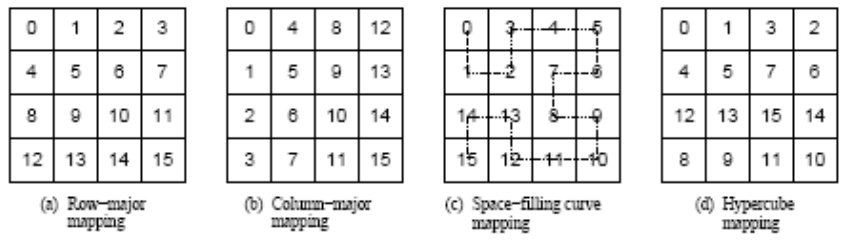
\includegraphics[height=0.3\textheight]{figures/MPI/Topology.png}
        \end{figure}
        \item Topology được xác định bởi chương trình, topology của máy vật lý
    \end{itemize}
\end{frame}

\begin{frame}{Topology theo tọa độ Decartes}
    \begin{itemize}
        \item Đối với các bài toán thông thường một tổ chức các tiến trình sử dụng mắt lưới ô vuông thường khá tự nhiên.
        \item Tạo một bộ giao tiếp với góc nhìn một ô lưới:
        \begin{itemize}
            \item int MPI\_Cart\_create(MPI\_Comm comm\_old, int ndims,
                                      int *dims, int *periods, int reorder,
                                      MPI\_Comm *comm\_cart)
            \item ndims: số chiều của ô lưới
            \item dims: vector là độ dài của từng chiều
            \item periods: vector biểu diễn chu kỳ của từng chiều
            \item reorder: float cho biết rank có thể thay đổi không
        \end{itemize}
        \item Tọa độ của tiến trình trong topology Decartes là vector ndims chiều
    \end{itemize}
\end{frame}

\begin{frame}{Topology theo tọa độ Decartes}
    \begin{itemize}
        \item Việc truyền, nhận thông điệp vẫn cần rank 1 chiều
        \item Ánh xạ tọa độ trên tọa độ Decarted $\Leftrightarrow$ rank:
        \begin{itemize}
            \item int MPI\_Cart\_coord(MPI\_Comm comm\_cart, int rank, int maxdims,
                                      int *coords) 
            \item int MPI\_Cart\_rank(MPI\_Comm comm\_cart, int *coords, int *rank) 
        \end{itemize}
        \item Phép toán hay được thực hiện trên topology Decarted nhất là phép dịch
        \item Xác định rank của tiến trình nguồn và tiến trình đích của một shift:
        \begin{itemize}
            \item int MPI\_Cart\_shift(MPI\_Comm comm\_cart, int dir, int s\_step,
                                       int *rank\_source, int *rank\_dest)
        \end{itemize}
    \end{itemize}
\end{frame}

\begin{frame}[shrink, fragile]{Topology theo tọa độ Decartes}
    \begin{verbatim}
int rank, size;
int dims[2] = {4, 4};  // Kích thước từng chiều
int periods[2] = {1, 0};  // Chu kỳ từng chiều
int coords[2];  // Tọa độ của tiến trình hiện tại trên ô lưới
int left, right, up, down;  // Các láng giềng trên ô lưới
...
MPI_Comm cart_comm;
MPI_Cart_create(MPI_COMM_WORLD, 2, dims, periods, 0, &cart_comm);
MPI_Cart_coords(cart_comm, rank, 2, coords);
MPI_Cart_shift(cart_comm, 0, 1, &left, &right);
MPI_Cart_shift(cart_comm, 1, 1, &up, &down); 
printf("Rank %d: Coordinates (%d, %d), 
        neighbors (left: %d, right: %d, up: %d, down: %d)\n",
        rank, coords[0], coords[1], left, right, up, down); 
MPI_Comm_free(&cart_comm);
MPI_Finalize();
    \end{verbatim}
\end{frame}

\begin{frame}{Chia topology Decartes}
    \begin{itemize}
        \item Các tiến trình được sắp xếp trên một ô lưới ảo sử dụng topology Decartes
        \item Đôi khi ta muốn hạn chế giao tiếp các tiến trình trên một tập hợp con của lưới.
        \item Chia topology Decartes thành các ô lưới có số chiều nhỏ hơn
        \begin{itemize}
            \item int MPI\_Cart\_sub(MPI\_Comm comm\_cart, int *keep\_dims,
                                     MPI\_Comm *comm\_subcart) 
        \end{itemize}
        \item Nếu keep\_dims[i] là true:
        \begin{itemize}
            \item Chiều thứ i được giữ lại trong topology nhỏ mới
        \end{itemize}
        \item Xử lý tọa độ trong topology nhỏ:
        \begin{itemize}
            \item Xuất phát từ tọa độ trong topology ban đầu
            \item Bỏ qua tọa độ cho các chiều đã bị loại bỏ
        \end{itemize}
    \end{itemize}
\end{frame}

\begin{frame}{Chia topology Decartes}
    \begin{figure}[H]
        \centering
        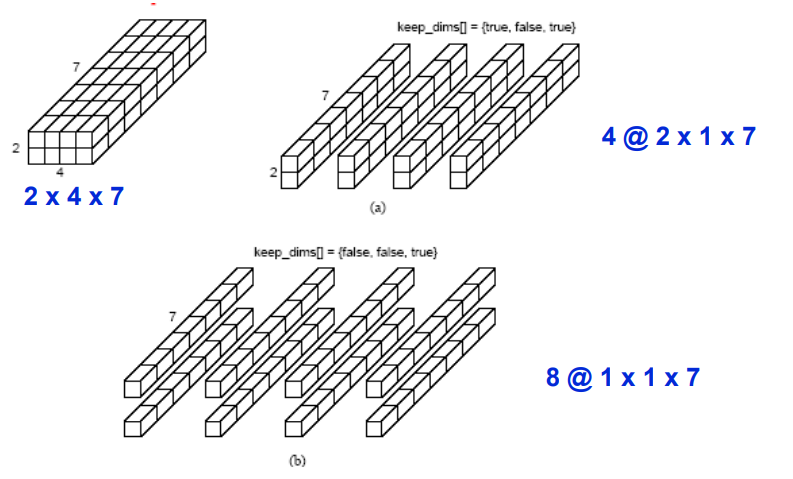
\includegraphics[height=0.6\textheight]{figures/MPI/Cartesion_sub.png}
        \caption{Ví dụ chia topology Decartes}
    \end{figure}
\end{frame}

\begin{frame}[shrink]{Topology đồ thị}
    \begin{itemize}
        \item Một số bài toán không thường gặp, việc tổ chức các tiến trình trên một đồ thị phù hợp:
        \begin{itemize}
            \item int MPI\_Graph\_create(MPI\_Comm comm\_old, int nnodes,
                                         int *index, int *edges,
                                         int reorder, MPI\_Comm *cgraph)           
        \end{itemize}
        \item nnodes: số đỉnh trong đồ thị (số tiến trình)
        \item index: vector các số nguyên biểu diễn bậc của các đỉnh
        \item edges: vector các số nguyên dạng danh sách kề
        \item reorder: float cho biết rank có thể thay đổi không
    \end{itemize}

    \begin{figure}[H]
        \centering
        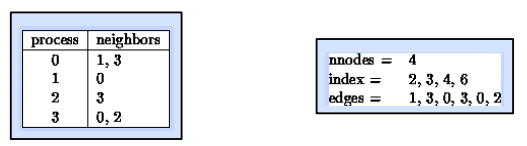
\includegraphics[height=0.3\textheight]{figures/MPI/Graph_Example.png}
    \end{figure}
\end{frame}

\begin{frame}[fragile]{Topology đồ thị}
    \begin{verbatim}
int rank, size;
int nnodes = 4;
int index[4] = {2, 2, 2, 2};
int edges[8] = {1, 3, 0, 2, 2, 0, 3, 1};
MPI_Comm comm_graph;
...
MPI_Graph_create(MPI_COMM_WORLD, nnodes, index, edges, 
                 0, &comm_graph);
int graph_rank, graph_size;
MPI_Comm_rank(comm_graph, &graph_rank);
MPI_Comm_size(comm_graph, &graph_size);
printf("Process %d (global rank) / %d (graph rank) 
        out of %d (global size) / %d (graph size)\n",
       rank, graph_rank, size, graph_size);
MPI_Comm_free(&comm_graph);
MPI_Finalize();
    \end{verbatim}
\end{frame}

\begin{frame}{Topology đồ thị}
    \begin{itemize}
        \item Truy vấn số đỉnh và vector cạnh
        \begin{itemize}
            \item int MPI\_Graphdims\_get(MPI\_Comm comm, int *nnodes,
                                         int *nedges)
        \end{itemize}
        \item Đọc cấu trúc danh sách kề qua index và edges
        \begin{itemize}
            \item int MPI\_Graph\_get(MPI\_Comm comm, int maxindex,
                                      int maxedges, int *index,
                                      int *edges)
        \end{itemize}
    \end{itemize}
\end{frame}

\subsection{Kiểu dữ liệu dẫn xuất trong trong MPI}

\begin{frame}{Kiểu dữ liệu dẫn xuất trong trong MPI}
    \begin{itemize}
        \item Một kiểu dữ liệu tổng quát là một đối tượng xác định hai yếu tố:
        \begin{itemize}
            \item Một dãy các kiểu dữ liệu cơ bản 
            \item Một dãy các số nguyên (số byte) là offset của các phần tử
        \end{itemize}
        \item Một số tính chất của kiểu dữ liệu tổng quát:
        \begin{itemize}
            \item Thứ tự của các phần tử không nhất thiết phải trùng với thứ tự của phần tử này trong bộ nhớ
            \item Một phần tử có thể xuất hiện nhiều lần
        \end{itemize}
        \item Ánh xạ kiểu dữ liệu: một cặp kiểu dữ liệu và offset
        \item Chữ ký kiểu dữ liệu: một dãy các kiểu dữ liệu cơ bản
    \end{itemize}
\end{frame}

\begin{frame}{Xây dựng kiểu dữ liệu dẫn xuất trong MPI}
    \begin{itemize}
        \item int MPI\_Type\_struct(int count, int blocklens[],
                                    MPI\_Aint indices[], MPI\_Datatype old\_types[],
                                    MPI\_Datatype *newtype )
        \item Nếu ta định nghĩa một kiểu dữ liệu có cấu trúc và muốn truyền nhận nhiều phần tử, ta đặt phần tử cuối cùng của mảng cấu trúc này là MPI\_UB.
    \end{itemize}
\end{frame}

\begin{frame}[shrink, fragile]{Xây dựng kiểu dữ liệu dẫn xuất trong MPI}
    \begin{verbatim}
typedef struct {
    int x;
    int y;
} Point;
Point p;
MPI_Datatype point_type;
int block_lengths[2] = {1, 1};
MPI_Aint displacements[2] = {0, sizeof(int)};
MPI_Datatype types[2] = {MPI_INT, MPI_INT};
MPI_Type_create_struct(2, block_lengths, displacements, 
types, &point_type);
MPI_Type_commit(&point_type);
if (rank == 0) {
    p.x = 10; p.y = 20;
    MPI_Send(&p, 1, point_type, 1, 0, MPI_COMM_WORLD);
} else if (rank == 1) {
    MPI_Recv(&p, 1, point_type, 0, 0, MPI_COMM_WORLD, MPI_STATUS_IGNORE);
}
    \end{verbatim}
\end{frame}

\begin{frame}[fragile]{Kiểu dữ liệu dẫn xuất trong trong MPI}
    \begin{itemize}
        \item int MPI\_Type\_contiguous(int count, MPI\_Datatype oldtype,
                                        MPI\_Datatype *newtype)
        \item Tạo ra kiểu dữ liệu mới newtype thu được bằng cách ghép count bản sao của kiểu dữ liệu cũ oldtype
       
    \end{itemize}
    \begin{verbatim}
int count = 3;
MPI_Datatype newtype;
MPI_Type_contiguous(count, MPI_INT, &newtype);
MPI_Type_commit(&newtype);
    \end{verbatim}
\end{frame}

\begin{frame}[fragile]{Kiểu dữ liệu dẫn xuất trong trong MPI}
    \begin{itemize}
        \item int MPI\_Type\_vector(int count, int blocklength, int stride,
                                    MPI\_Datatype oldtype,
                                    MPI\_Datatype *newtype)
    \end{itemize}

    \begin{verbatim}
int rows = 2;
int cols = 3;
int stride = cols + 1;  // Stride of 1 row + 1 column
int data[rows][cols] = {{1, 2, 3}, {4, 5, 6}};
MPI_Datatype newtype;
MPI_Type_vector(rows, cols, stride, MPI_INT, &newtype);
MPI_Type_commit(&newtype);
    \end{verbatim}
\end{frame}

\begin{frame}{MPI Runtime}
    \begin{itemize}
        \item Cung cấp các tiến trình thực thi và xử lý tín hiệu
        \item Xử lý tín hiệu (SIGKILL, SIGSUSP, SIGUSR1/2)
        \item Thu thập stdout và stderr, lan truyền stdin
        \item Có thể lan truyền các biến môi trường 
        \item Cung cấp các gói hỗ trợ cho debug, profile, truy vết 
        \item Có thể giao tiếp với một hệ thống hàng đợi để sắp xếp các tiến trình tốt hơn
        \item MPI-2 phát triển một bản sao của mpirun được chuẩn hóa: mpiexec
        \item Các tham số dòng lệnh và các biến môi trường cho phép linh hoạt thực thi chương trình
    \end{itemize}
\end{frame}

\begin{frame}{Môi trường MPI}
    \begin{itemize}
        \item Thực hiện chức năng khởi tạo, kết thúc hoặc hủy bỏ
        \item Xử lý lỗi (ngoại lệ)
        \item Một số hàm cần thiết:
        \begin{itemize}
            \item double MPI\_Wtime(void), double MPI\_Wtick(void)
            \item MPI\_Get\_processor\_name(char *name, int *resultlen)
        \end{itemize}
        \item Hàm truy vấn communicator (size, rank) cho MPI\_COMM\_WORLD
    \end{itemize}

\end{frame}

\begin{frame}{Xử lý ngoại lệ}
    \begin{itemize}
        \item Sử dụng các hàm xử lý ngoại lệ và các MPI return codes
        \item Bộ xử lý lỗi mặc định: MPI\_ERRORS\_ARE\_FATAL
        \begin{itemize}
            \item Bộ xử lý lỗi khi được gọi sẽ làm chương trình hủy bỏ thực thi tất cả các tiến trình hiện tại.
            Cùng hiệu ứng tương tự như MPI\_ABORT được gọi bởi tiến trình gọi Bộ xử lý lỗi
        \end{itemize}
        \item Bộ xử lý lỗi thay thế: MPI\_ERRORS\_RETURN
        \begin{itemize}
            \item Bộ xử lý lỗi chỉ trả về mã lỗi cho người dùng
            \item MPICH cung cấp thêm 2 tính tăng:
            \begin{itemize}
                \item MPE\_Errors\_call\_dbx\_in\_xterm
                \item MPE\_Signals\_call\_debugger 
            \end{itemize}
        \end{itemize}
    \end{itemize}
\end{frame}

\begin{frame}{Xử lý lỗi}
    \begin{itemize}
        \item Một số hàm xử lý lỗi:
        \begin{itemize}
            \item MPI\_Errhandler\_create(MPI\_Handler\_function *function,
                                          MPI\_Errhandler *errhandler) 
            \item MPI\_Errhandler\_set(MPI\_Comm comm, MPI\_Errhandler errhandler) 
            \item MPI\_Errhandler\_get(MPI\_Comm comm, MPI\_Errhandler *errhandler)
            \item MPI\_Errhandler\_free(MPI\_Errhandler *errhandler)
            \item MPI\_Error\_string(int errorcode, char *string, int *resultlen)
            \item MPI\_Error\_class(int errorcode, int *errorclass)
        \end{itemize}
    \end{itemize}
\end{frame}

\begin{frame}{Các công cụ profile}
    \begin{itemize}
        \item Tất cả các hàm profile sử dụng tiền tối PMPI\_... 
        \item Thư viện profile có thể viết riêng hàm MPI\_ và gọi hàm PMPI\_ tương ứng để thực hiện truyền thông điệp
        \item Cung cấp một cách truy vết cũng như profile về chi phí thời gian thực thi một chương trình song song khi cần cải thiện hiệu năng hoặc lỗi logic
    \end{itemize}
\end{frame}

\section{CUDA}

\subsection{Tổng quan kiến trúc GPU}

\begin{frame}{Định luật Moore}
    \begin{itemize}
        \item Số bóng bán dẫn trên một vi mạch sẽ tăng gấp đôi sau mỗi hai năm
    \end{itemize}
    \begin{figure}[H]
        \centering
        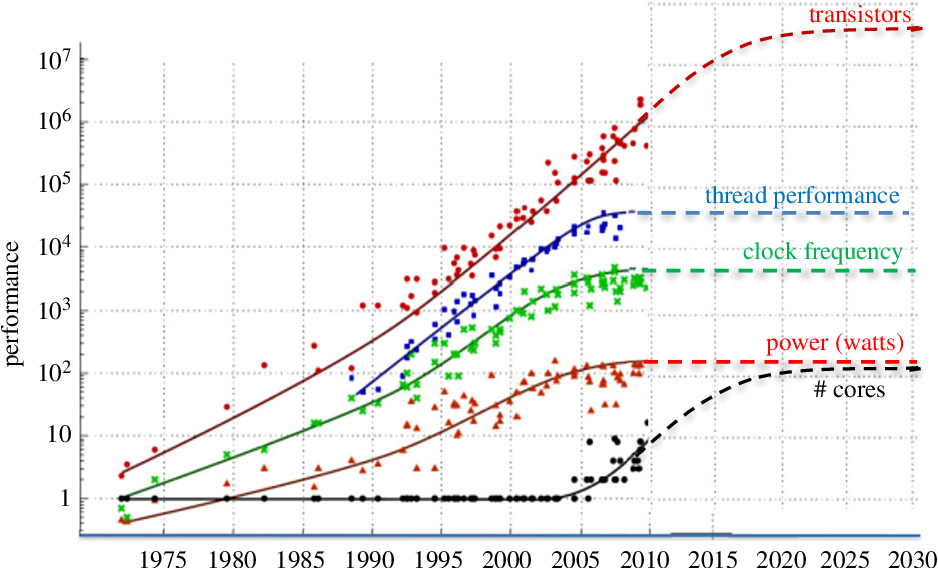
\includegraphics[height=0.7\textheight]{figures/CUDA/Moore_Law.png}
    \end{figure}
\end{frame}

\begin{frame}{Định luật Moore}
    \begin{itemize}
        \item Khả năng tích hợp bóng bán dẫn trên một vi mạch dần bị bão hòa
        \item Vi xử lý gần như không thể nhanh hơn
        \item Phát triển theo hướng song song
    \end{itemize}
\end{frame}

\begin{frame}{Các hệ thống siêu máy tính dùng CPU}
    \begin{itemize}
        \item Chi phí đắt
        \item Kích thước lớn
        \item Chỉ có thể hoạt động tin cậy sau khi chạy chương trình vài giờ
    \end{itemize}
\end{frame}

\begin{frame}{Graphic Processing Units (GPU)}
    \begin{itemize}
        \item GPU (Graphical Processing Unit) là một loại phần cứng được thiết kế chuyên dụng cho các ứng dụng tính toán song song (đồ họa)
    \end{itemize}
    \begin{figure}[H]
        \centering
        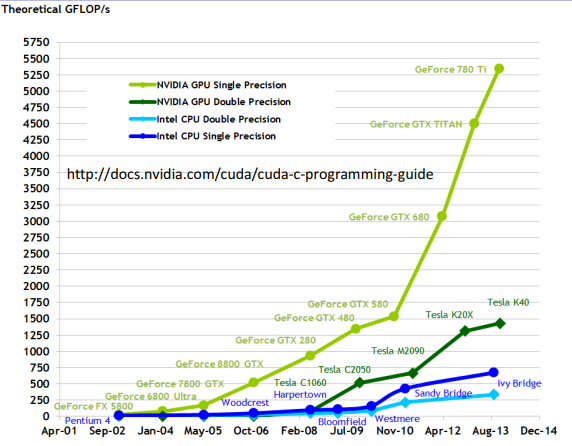
\includegraphics[height=0.7\textheight]{figures/CUDA/GFLOP_Trend.png}
    \end{figure}
\end{frame}

\begin{frame}{Graphic Processing Units (GPU)}
    \begin{itemize}
        \item Tốc độ xử lý nhanh cần có băng thông lớn
    \end{itemize}
    \begin{figure}[H]
        \centering
        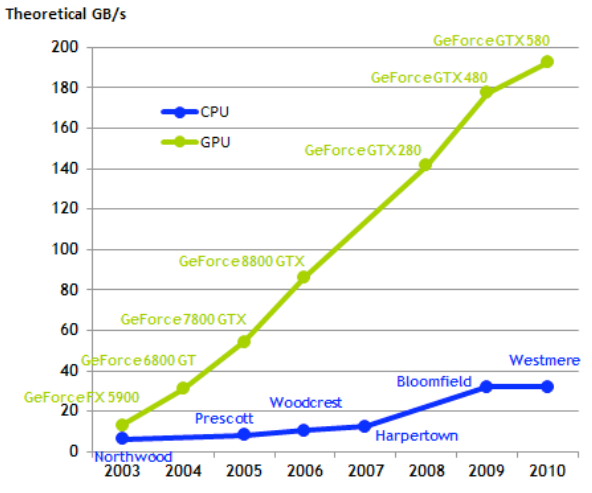
\includegraphics[height=0.7\textheight]{figures/CUDA/Bandwidth.png}
    \end{figure}
\end{frame}

\begin{frame}{Thiết kế CPU và GPU}
    \begin{figure}[H]
        \centering
        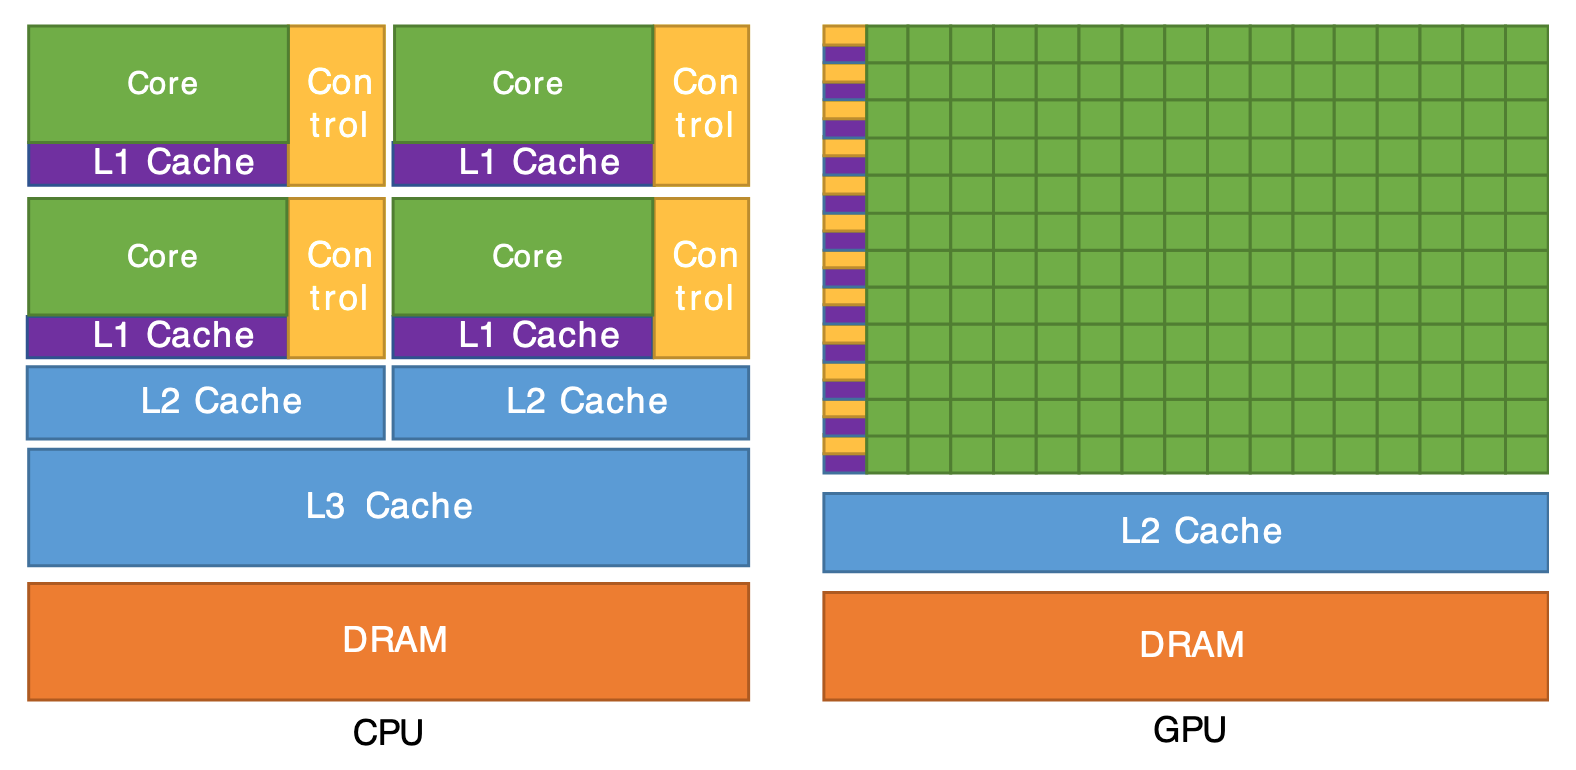
\includegraphics[height=0.7\textheight]{figures/CUDA/CPUvsGPU_design.png}
        caption{So sánh thiết kế CPU và GPU}
    \end{figure}
\end{frame}

\begin{frame}{Tính toán trên GPU}
    \begin{itemize}
        \item Ban đầu, GPU chỉ phục vụ cho việc tính toán ứng dụng liên quan đến đồ họa
        \item GPU dần cũng được sử dụng cho các ứng dụng xử lý ảnh
        \item Dần được phục vụ cho các tác vụ tính toán nói chung khi dữ liệu có thể chia tách và xử lý song song
    \end{itemize}
\end{frame}

\begin{frame}{Kết nối CPU và GPU}
    \begin{itemize}
        \item GPU được kết nối với CPU qua một bus tốc độ cao (PCI Express)
    \end{itemize}
    \begin{columns}[onlytextwidth]
        \begin{column}{0.35\linewidth}
            \begin{figure}[H]
                \centering
                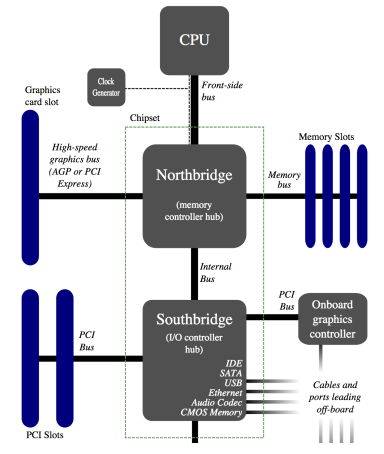
\includegraphics[width=\linewidth]{figures/CUDA/Mainboard.png}
                \caption{Sơ đồ của mainboard}
            \end{figure}
        \end{column}
        \begin{column}{0.65\linewidth}
            \begin{figure}[H]
                \centering
                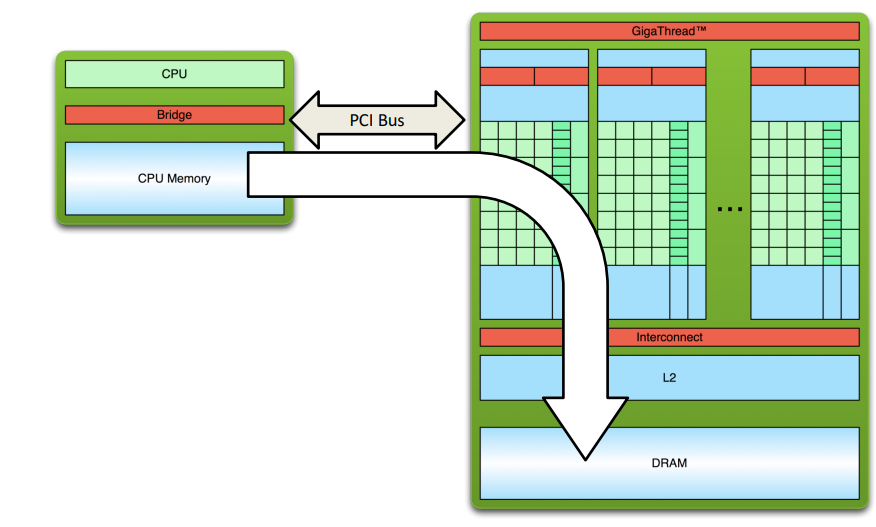
\includegraphics[width=\linewidth]{figures/CUDA/PCIe.png}
            \end{figure}
        \end{column}
    \end{columns}
\end{frame}

\begin{frame}{Thiết kế của GPU}
    \begin{itemize}
        \item GPU gồm rất nhiều lõi, mỗi lõi được gọi là stream processor.
        \item Các stream processors được chia thành các nhóm được gọi là Stream Multiprocessors (SMs)
        \item SMs cơ bản là một bộ xử lý SIMD
    \end{itemize}
    \begin{figure}[H]
        \centering
        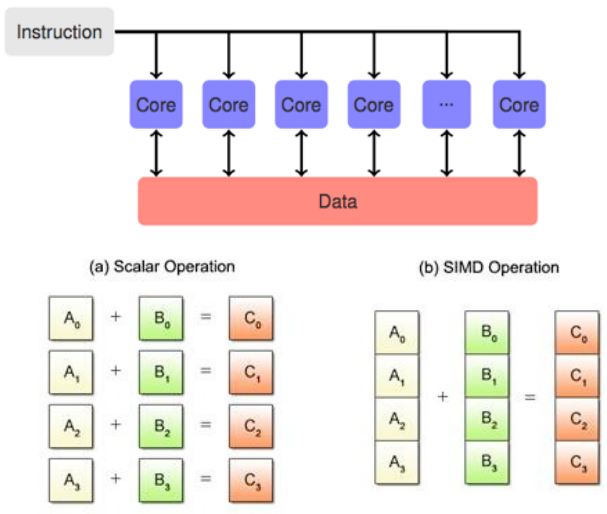
\includegraphics[height=0.5\textheight]{figures/CUDA/SIMD.png}
    \end{figure}
\end{frame}

\begin{frame}{Thiết kế của GPU}
    \begin{itemize}
        \item GPU bao gồm nhiều lõi đơn giản
        \item Được thiết kế cho nhiều tác vụ đơn giản: thông lượng dữ liệu cao
        \item Ít control units: giảm độ trễ (latency)
    \end{itemize}
\end{frame}

\subsection{Computing Unified Device Architecture (CUDA)}

\begin{frame}{Computer Unified Device Architecture (CUDA)}
    \begin{itemize}
        \item Là kiến trúc và mô thức lập trình
        \item Kiến trúc và mô hình thực things
        \begin{itemize}
            \item Được NVIDIA giới thiệu vào năm 2006
            \item Để có hiệu năng chương trình cao nhất yêu cầu cần hiểu kiến trúc phần cứng
        \end{itemize}
        \item Mô thức lập trình:
        \begin{itemize}
            \item Một tập nhỏ mở rộng của C
            \item Cho phép GPU thực thi chương trình được viết bằng C
            \item Trong chương trình C, gọi hàm SIMD"kernel" được thực thi trên GPU
        \end{itemize}
        \item Cần phải quản lý bộ nhớ GPU tương đối thủ công
    \end{itemize}
\end{frame}

\begin{frame}{CUDA}
    \begin{itemize}
        \item Một số thuật ngữ trong CUDA:
        \begin{itemize}
            \item Host: CPU và bộ nhớ của CPU (host memory)
            \item Device: GPU và bộ nhớ của GPU (device memory)
        \end{itemize}
    \end{itemize}
\end{frame}

\begin{frame}{Các bước chính trong một chương trình CUDA}
    \begin{enumerate}
        \item Cấp phát và khởi tạo các biến trên host và device
        \item Chuyển dữ liệu từ host sang device
        \item Thực hiện tính toán trên device
        \item Chuyển kết quả từ device sang host
        \item Giải phóng các vùng nhớ đã được cấp phát trên host và device
    \end{enumerate}
\end{frame}

\begin{frame}[fragile]{Biên dịch và chạy chương trình CUDA}
    \begin{itemize}
        \item Phải cài CUDA SDK và NVIDIA Graphic Driver
        \item Dùng trình biên dịch NVIDA: nvcc
    \end{itemize}
    \begin{verbatim}
__global__ void hellokernel() {
    printf(”Hello World!\n”);
}
int main(void){
    int num_threads = 1;
    int num_blocks = 1;
    hellokernel<<<num_blocks,num_threads>>>();
    cudaDeviceSynchronize();
    return 0;
}
    \end{verbatim}
    \begin{verbatim}
nvcc hello.cu -o a.out && ./a.out
    \end{verbatim}
\end{frame}

\begin{frame}{Mô hình thực thi}
    \begin{figure}[H]
        \centering
        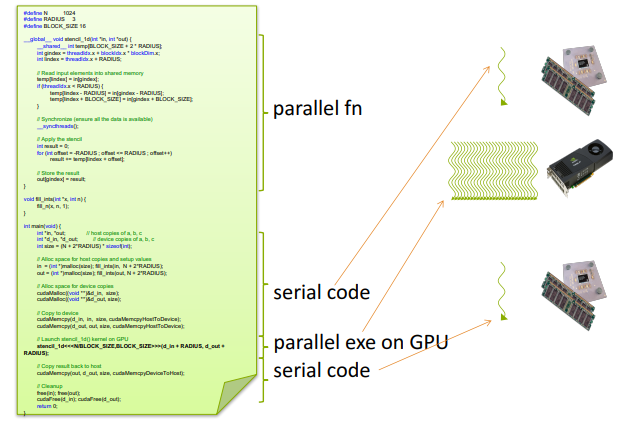
\includegraphics[width=0.8\linewidth]{figures/CUDA/Execution_Model.png}
        \caption{Trình tự thực thi chương trình CUDA}
    \end{figure}
\end{frame}

\subsection{Tổ chức phân cấp luồng trong CUDA}

\begin{frame}{Luồng trong CUDA}
    \begin{columns}[onlytextwidth]
        \begin{column}{0.5\linewidth}
            \begin{itemize}
                \item Các luồng được phân nhóm thành các thread blocks:
                \begin{itemize}
                    \item Tất cả các luồng trong một thread block chạy trên một một SMs
                    \item Các luồng trong cùng một block có thể giao tiếp
                    \item Cho phép xử lý hiệu quả trê dữ liệu 1-D, 2-D, 3-D
                \end{itemize}
                \item Nhiều thread block tạo nên một grid
            \end{itemize}
        \end{column}
        \begin{column}{0.5\linewidth}
            \begin{figure}[H]
                \centering
                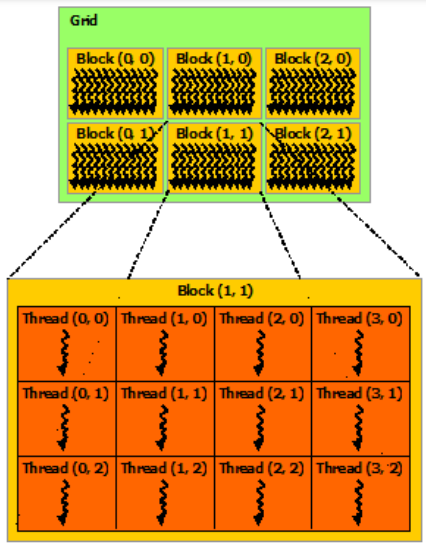
\includegraphics[height=0.8\textheight]{figures/CUDA/Thread_Hierachy.png}
            \end{figure}
        \end{column}
    \end{columns}
\end{frame}

\begin{frame}{Luồng trong CUDA}
    \begin{itemize}
        \item CUDA ảo hóa phần cứng vật lý
        \begin{itemize}
            \item Luồng là một bộ xử lý số vô hướng ảo hóa
            \item Các thread block là một bộ đa xử lý ảo hóa
        \end{itemize}
        \item Các thread block độc lập với nhau, không liên quan đến thứ tự
    \end{itemize}
\end{frame}


\begin{frame}{Luồng trong CUDA}
    \begin{columns}[onlytextwidth]
        \begin{column}{0.5\linewidth}
            \begin{itemize}
                \item Cung cấp tính năng tự động mở rộng trong GPU
                \begin{itemize}
                    \item Phân cấp luồng
                    \item Bộ nhớ chia sẻ
                    \item Đồng bộ luồng
                \end{itemize}
            \end{itemize}
        \end{column}
        \begin{column}{0.5\linewidth}
            \begin{figure}[H]
                \centering
                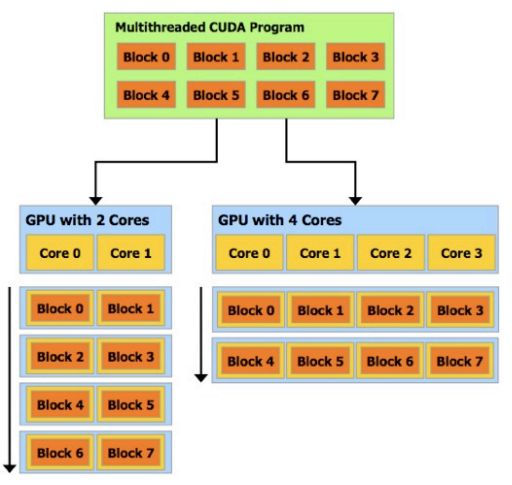
\includegraphics[width=\linewidth]{figures/CUDA/Multithread_SM.png}
            \end{figure}
        \end{column}
    \end{columns}
\end{frame}

\begin{frame}{Luồng trong CUDA}
    \begin{itemize}
        \item Mỗi luồng có một ID riêng tạo nên từ tổ hợp gồm blockID và threadID
        \item Ta có thể tính toán dữ liệu trên các phần khác nhau của dữ liệu
        \item SIMT: Single Instruction Multiple threads
        \item Threads: 1D, 2D, 3D
        \item Blocks: 1D, 2D
    \end{itemize}
\end{frame}

\begin{frame}[shrink]{CUDA - Mở rộng của C}
    \begin{itemize}
        \item Khai báo hàm:
        \begin{itemize}
            \item \_\_global\_\_ void kernel();
            \item \_\_device\_\_ float function();
        \end{itemize}
        \item Hạn định biến:
        \begin{itemize}
            \item \_\_shared\_\_ float array[5];
            \item \_\_constant\_\_ float array[5];
        \end{itemize}
        \item Cấu hình kernel:
        \begin{itemize}
            \item dim3 dim\_grid(100, 100); // 10000 blocks
            \item dim3 dim\_block(16, 16); // 256 threads per block in 2D
            \item kernel<<<dim\_grid, dim\_block>>>(); // Launch kernel
        \end{itemize}
        \item Các biến built-in: threadIdx.x, blockIdx.x
    \end{itemize}
\end{frame}

\begin{frame}{CUDA - Mở rộng của C}
    \begin{itemize}
        \item Từ khóa CUDA C/C++: \_\_global\_\_ biểu thị một hàm:
        \begin{itemize}
            \item Chạy trên device 
            \item Được gọi từ host code
        \end{itemize}
        \item Cặp 3 dấu ngoặc nhọn đánh dấu lời gọi từ host sang device:
        \begin{itemize}
            \item Còn được gọi là "kernel launch"
            \item Các tham số trong < < <...> > > là cấu hình các thread
        \end{itemize}
        \item nvcc chia code thành code của host và device:
        \begin{itemize}
            \item Hàm trên device (hellokernel()) được xử lý bởi trình biên dịch của NVIDIA
            \item Hàm host (main()) được xử lý bởi trình biên dịch tiêu chuẩn (gcc, cl.exe)
        \end{itemize}
    \end{itemize}
\end{frame}

\subsection{Mô hình thực thi trên GPU}

\begin{frame}{Mô hình thực thi trên GPU}
    \begin{columns}[onlytextwidth]
        \begin{column}{0.5\linewidth}
            \begin{itemize}
                \item Gồm nhiều lõi đơn giản
                \item Ví dụ Kiến trúc Fermi:
                \begin{itemize}
                    \item 16 SMs:
                    \begin{itemize}
                        \item 32 core 
                        \item Shared memory, registers, cache 
                        \item SFU, CU
                        \item 1TFLOP 
                        \item 144GB/s bandwidth
                    \end{itemize}
                \end{itemize}
            \end{itemize}
        \end{column}
        \begin{column}{0.5\linewidth}
            \begin{figure}[H]
                \centering
                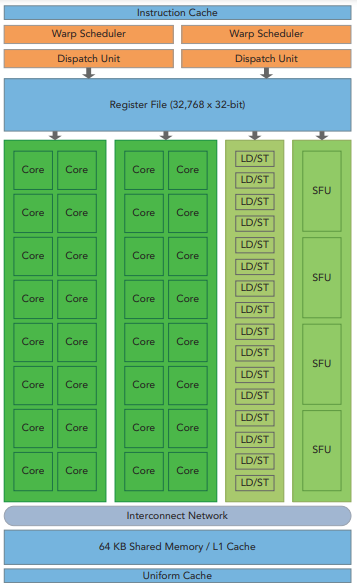
\includegraphics[width=0.75\linewidth]{figures/CUDA/SMs_diagram.png}
            \end{figure}
        \end{column}
    \end{columns}
\end{frame}

\begin{frame}{Mô hình thực thi trên GPU}
    \begin{figure}[H]
        \centering
        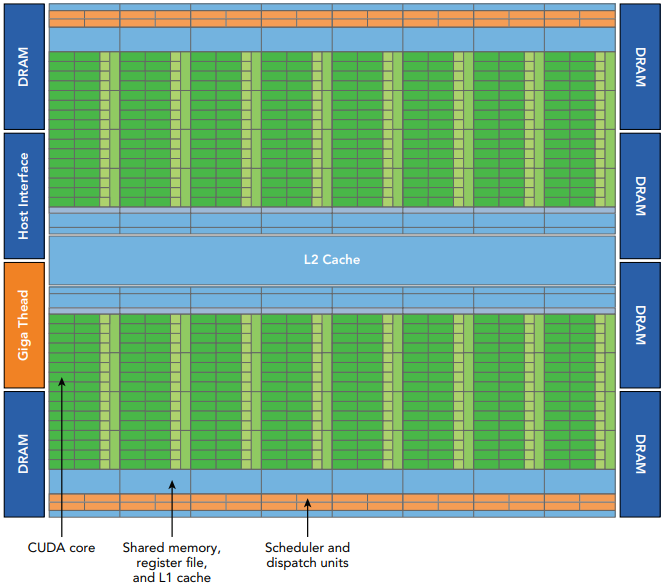
\includegraphics[width=0.65\linewidth]{figures/CUDA/Fermi_Architecture.png}
        \caption{Sơ đồ GPU kiến trúc Fermi}
    \end{figure}
\end{frame}

\begin{frame}{Mô hình thực thi trên GPU}
    \begin{figure}[H]
        \centering
        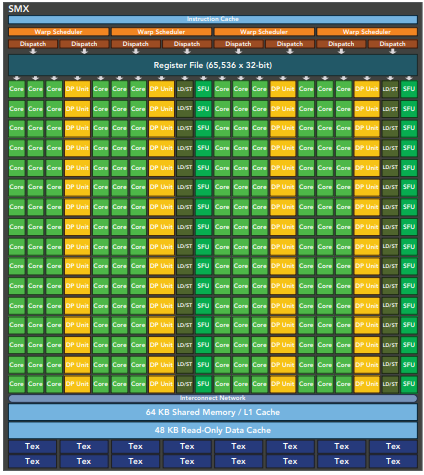
\includegraphics[width=0.45\linewidth]{figures/CUDA/SM_Kepler_Architecture.png}
        \caption{Sơ đồ SM kiến trúc Kepler}
    \end{figure}
\end{frame}

\begin{frame}{Mô hình thực thi trên GPU}
    \begin{figure}[H]
        \centering
        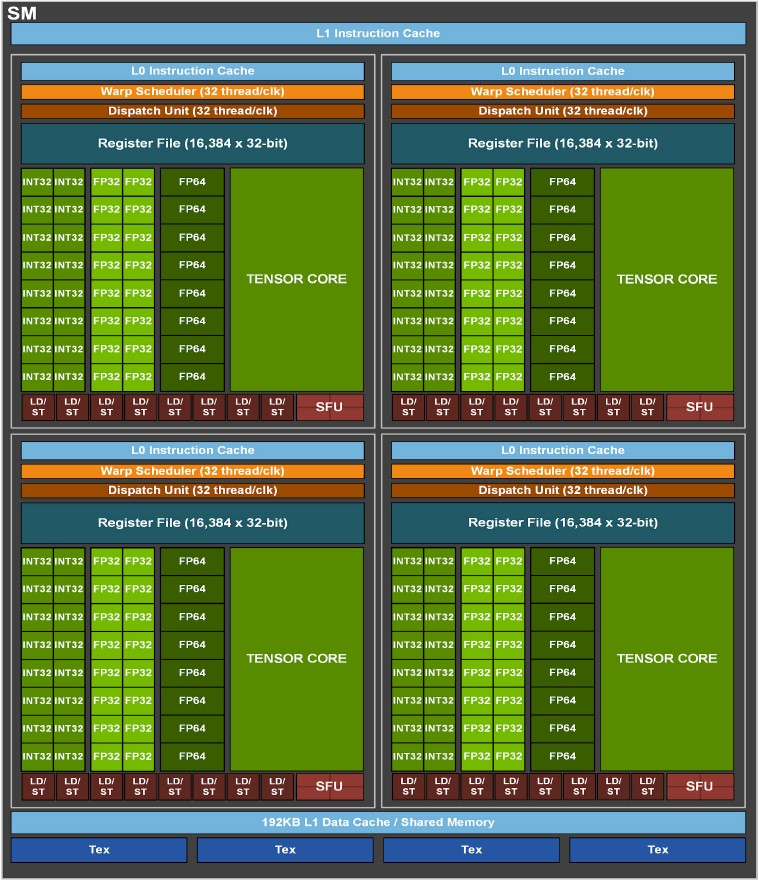
\includegraphics[width=0.45\linewidth]{figures/CUDA/SM_Hopper_Archtecture.jpg}
        \caption{Sơ đồ SM kiến trúc Hopper}
    \end{figure}
\end{frame}

\begin{frame}{Mô hình thực thi trên GPU}
    \begin{itemize}
        \item Các đặc điểm của luồng trong CUDA
        \begin{itemize}
            \item Mỗi luồng có một bộ đếm địa chỉ chương trình riêng
            \item Mỗi luồng có một tập thanh ghi riêng
            \item Mỗi luồng có một đường đi thực thi riêng
        \end{itemize}
    \end{itemize}
\end{frame}

\begin{frame}{Mô hình thực thi trên GPU}
    \begin{figure}[H]
        \centering
        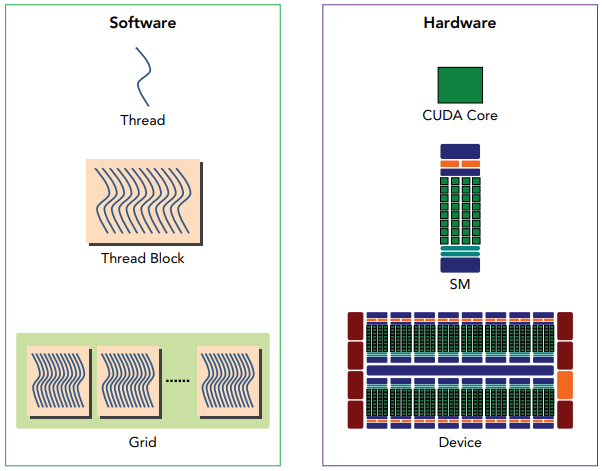
\includegraphics[width=0.7\linewidth]{figures/CUDA/Software_vs_Hardware.png}
    \end{figure}
\end{frame}

\begin{frame}{Mô hình thực thi trên GPU}
    \begin{itemize}
        \item Khi chương trình gọi kernel, các thread block sẽ được đặt lịch trình vào một SMs.
        \item Thread block sẽ ở trên SMs đến khi được thực thi xong hết
        \item Một SM có thể được gán nhiều thread block
        \item Từng luồng sẽ được gán một lượng tài nguyên (số thanh ghi, bộ nhớ cục bộ)
    \end{itemize}
\end{frame}

\begin{frame}{Mô hình thực thi trên GPU}
    \begin{figure}[H]
        \centering
        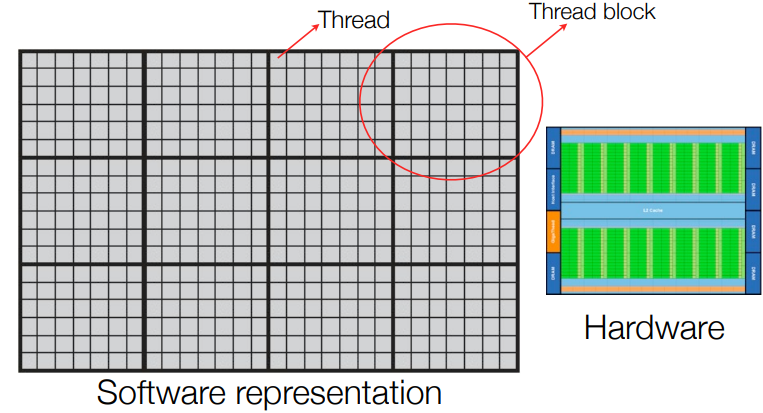
\includegraphics[width=0.85\linewidth]{figures/CUDA/Connecting_SW_HW_1.png}
    \end{figure}
\end{frame}

\begin{frame}{Mô hình thực thi trên GPU}
    \begin{itemize}
        \item Phần cứng sẽ lên lịch trình các thread block vào các SMs còn vị trí cho các block 
        \item Không có thứ tự thực hiện rõ ràng
        \item Nếu một SMs có nhiều tài nguyên hơn thì phần cứng sẽ ưu tiên lên lịch trình block vào SMs này
    \end{itemize}
\end{frame}

\begin{frame}{Mô hình thực thi trên GPU}
    \begin{figure}[H]
        \centering
        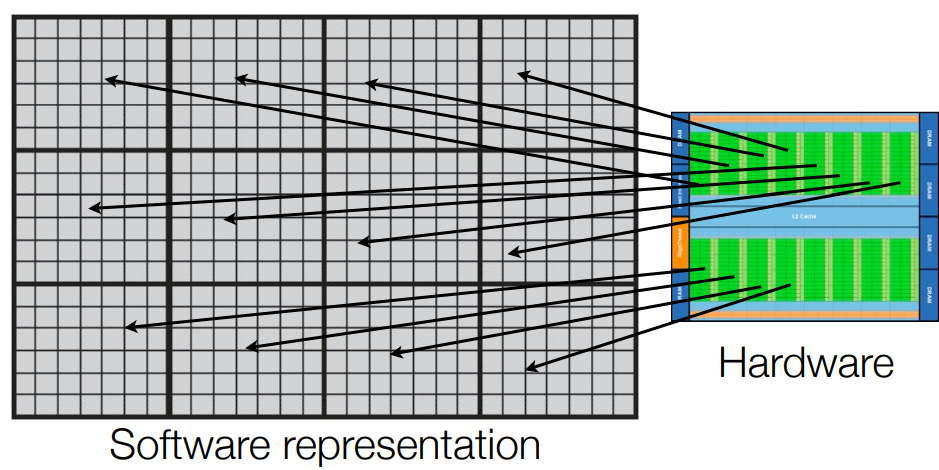
\includegraphics[width=0.85\linewidth]{figures/CUDA/Connecting_SW_HW_2.png}
    \end{figure}
\end{frame}

\begin{frame}[shrink]{Warps}
    \begin{itemize}
        \item Về mặt logic, các luồng trong cùng một block thực thi song song. Nhưng về mặt phần cứng thì không
        \item CUDA thực hiện kiến trúc SIMT (Single Instruction Multiple Thread) để quản lý và thực thi các luồng trong một nhóm 32 luồng gọi là warps.
        \item Các luồng trong cùng một warp thực thi cùng một chương trình tại một thời điểm
        \item Không có thứ tự thực hiện rõ ràng từ trước
    \end{itemize}

    \begin{figure}[H]
        \centering
        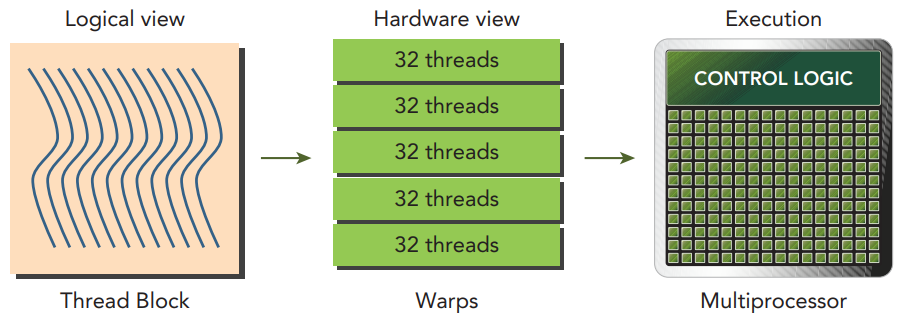
\includegraphics[width=0.7\linewidth]{figures/CUDA/Logical_view_vs_Hardware_view.png}
    \end{figure}
\end{frame}

\begin{frame}{Warps}
    \begin{columns}[onlytextwidth]
        \begin{column}{0.5\linewidth}
            \begin{itemize}
                \item Các luồng trong một warp bắt buộc phải cùng một block 
                \item Các luồng trong warp được gán từ các luồng có id liền nhau trong một block 
            \end{itemize}
        \end{column}\begin{column}{0.5\linewidth}
                \begin{figure}[H]
                    \centering
                    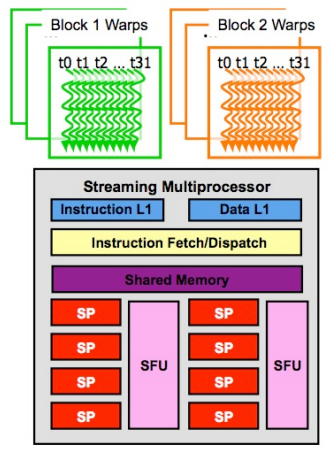
\includegraphics[width=0.8\linewidth]{figures/CUDA/SIMT_Warps.png}
                \end{figure}
        \end{column}
    \end{columns}
\end{frame}

\begin{frame}{Warps}
    \begin{columns}[onlytextwidth]
        \begin{column}{0.5\linewidth}
            \begin{itemize}
                \item Kiến trúc Fermi, mỗi SMs có:
                \begin{itemize}
                    \item Hai warp scheduler
                    \item Hai đơn vị thực thi chương trình
                \end{itemize}
                \item Kiến trúc Kepler, mỗi SMs có:
                \begin{itemize}
                    \item 4 Warp schduler
                    \item 8 đơn vị thực thi chương trình
                \end{itemize}
            \end{itemize}
        \end{column}
        \begin{column}{0.5\linewidth}
            \begin{figure}[H]
                \centering
                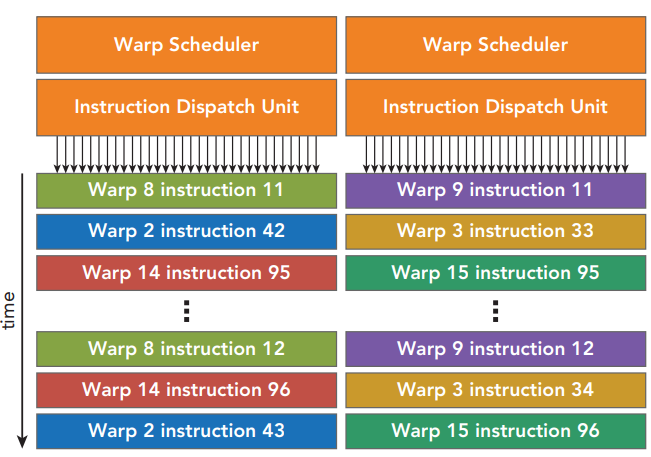
\includegraphics[width=\linewidth]{figures/CUDA/Warp_Scheduler.png}
            \end{figure}
        \end{column}
    \end{columns}
\end{frame}

\begin{frame}{Warps}
    \begin{itemize}
        \item SMs gần như không tốn chi phí cho việc lên lịch trình thực thi các warps
        \item Các warp đã sẵn sàng về dữ liệu, chương trình và có vẫn còn đủ CUDA core trong SM được gọi là eligible
        \item Các eligible warp sẽ được ưu tiên trong lên lịch trình thực thi 
    \end{itemize}

    \begin{figure}[H]
        \centering
        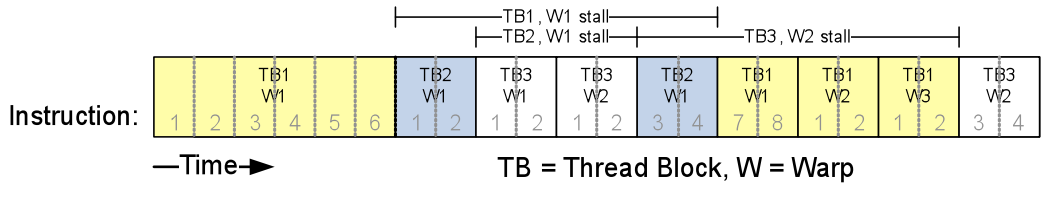
\includegraphics[width=0.8\linewidth]{figures/CUDA/Eligible_Stall_Warps.png}
    \end{figure}
\end{frame}

\begin{frame}{Warp Divergence}
    \begin{itemize}
        \item Tránh tối đa việc sử dụng if - else, for, while trong kernel 
    \end{itemize}
    \begin{figure}[H]
        \centering
        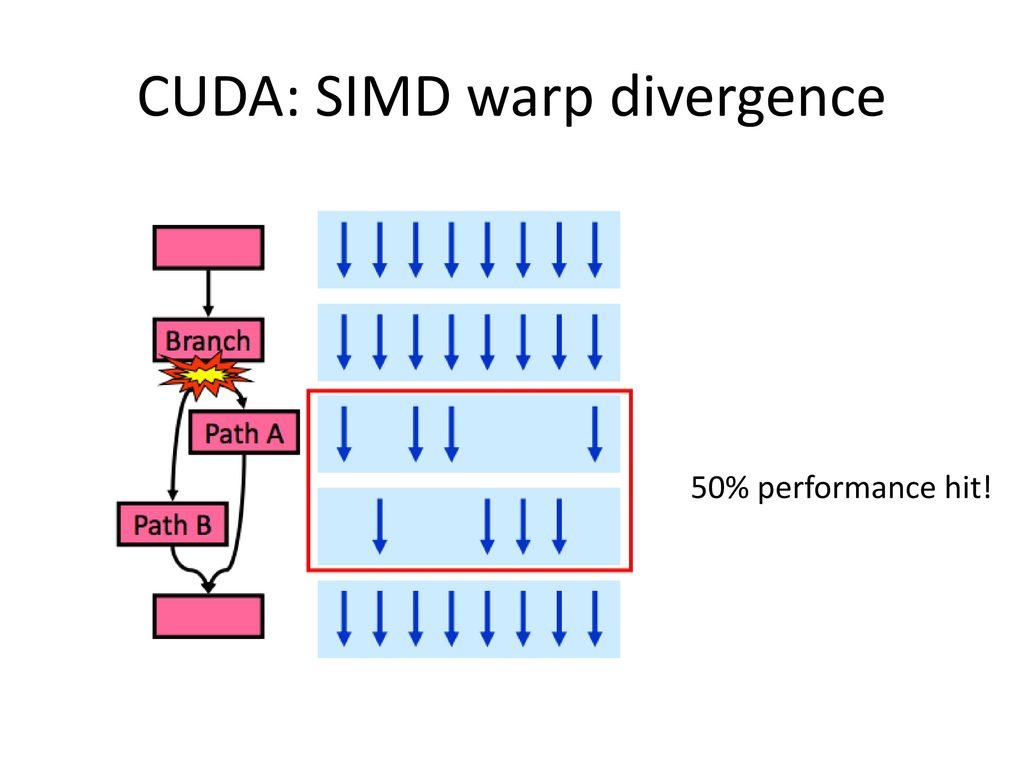
\includegraphics[width=0.7\linewidth]{figures/CUDA/Warp_Divergence.jpg}
    \end{figure}
\end{frame}

\subsection{Điều khiển GPU}

\begin{frame}[fragile]{Điều khiển GPU}
    \begin{itemize}
        \item CUDA kernel:
        \begin{itemize}
            \item Định nghĩa tác vụ được thực thi bởi một luồng đơn trên GPU
            \item Cách viết tương tự như cách viết hàm trên CPU
            \item Cú pháp của một kernel cũng tương tự một hàm trên C/C++ nhưng thêm:
            \begin{verbatim}
__global__ void kernel(...) {
    ...
}
            \end{verbatim}
            \item Mọi luồng CUDA thực thi cùng một kernel (SIMT)
            \item Ban đầu, điểm khác biệt duy nhất giữa các luồng là tọa độ của luồng
        \end{itemize}
    \end{itemize}
\end{frame}

\begin{frame}[fragile]{Tổ chức luồng trong GPU}
    \begin{itemize}
        \item Phân cấp luồng trong CUDA 
        \begin{itemize}
            \item Warp: Một group SIMT
            \item Thread block: một vài nhóm SIMT chạy đồng thời trên một SMs
            \item Grid: tất cả các thread block được tạo bởi cùng kernel launch
        \end{itemize}
        \item Launch một kernel tương tự như gọi hàm:
        \begin{itemize}
            \item Tên kernel và các tham Số
            \item Số thread block trên một grid và và số thread trên một block được tạo ra:
            \begin{verbatim}
kernel<<<nblocks, threads_per_block>>>(arg1, arg2, ...);                
            \end{verbatim}
        \end{itemize}
    \end{itemize}
\end{frame}

\begin{frame}[fragile]{Tổ chức luồng trong GPU}
    \begin{itemize}
        \item Các luồng của GPU có thể cấu hình 1-D, 2-D, 3-D
        \item Block và Grid đều 1 chiều:
    \end{itemize}
    \begin{verbatim}
int nblocks = 4;
int threads_per_block = 8;
kernel<<<nblocks, threads_per_block>>>(...);
    \end{verbatim}

    \begin{figure}[H]
        \centering
        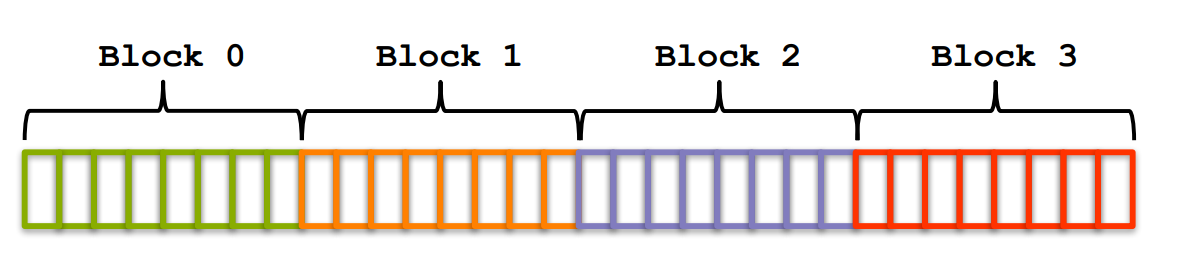
\includegraphics[width=0.7\linewidth]{figures/CUDA/1d_Grid_Block.png}
    \end{figure}
\end{frame}

\begin{frame}[fragile]{Tổ chức luồng trong GPU}
    \begin{itemize}
        \item Block và Grid đều 2 chiều:
    \end{itemize}
    \begin{verbatim}
dim3 nblocks(2,2);
int threads_per_block = 8;
kernel<<<nblocks, threads_per_block>>>(...);
    \end{verbatim}

    \begin{figure}[H]
        \centering
        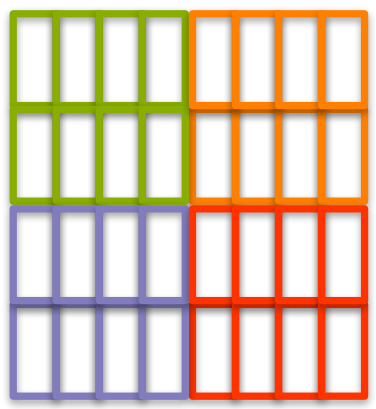
\includegraphics[height=0.5\textheight]{figures/CUDA/2d_Grid_Block.png}
    \end{figure}
\end{frame}

\begin{frame}[fragile]{Tổ chức luồng trong GPU}
    \begin{itemize}
        \item Block 1 chiều và Grid 2 chiều:
    \end{itemize}

    \begin{verbatim}
dim3 nblocks(2,2);
int threads_per_block = 8;
kernel<<<nblocks, threads_per_block>>>(...);
    \end{verbatim}

    \begin{figure}[H]
        \centering
        \includegraphics[width=0.7\linewidth]{figures/CUDA/2d_1d_Grid_Block.png}
    \end{figure}
\end{frame}

\begin{frame}{Tổ chức luồng trong GPU}
    \begin{itemize}
        \item Trên GPU, số block và thread trên một block được hiển thị qua các biến tọa độ luồng:
        \begin{itemize}
            \item Kích thước Chiều
            \item IDs
        \end{itemize}
        \begin{table}[H]
            \centering
            \resizebox{\columnwidth}{!} {
                \begin{tabular}{|l|l|}
                    \hline
                    Tên biến & Ý nghĩa \\
                    \hline
                    gridDim.x, gridDim.y, gridDim.z & Số block theo từng trục trong kernel launch \\
                    \hline
                    blockIdx.x, blockIdx.y, blockIdx.z & ID của block đang chứa thread hiện tại \\
                    \hline
                    blockDim.x, blockDim.y, blockDim.z & Số luồng trong một block \\
                    \hline
                    threadIdx.x, threadIdx.y, threadIx.z & ID của luồng hiện tại trong block chứa luồng này \\
                    \hline
                \end{tabular}
            }
        \end{table}
    \end{itemize}

\end{frame}


\begin{frame}{Tổ chức luồng trong GPU}
    \begin{itemize}
        \item Để tính ID toàn cục của một luồng trên GPU trong một grid 1 chiều và block 1 chiều:
    \end{itemize}
    \begin{figure}[H]
        \centering
        \includegraphics[height=0.6\textheight]{figures/CUDA/Global_ThreadID_1d_Grid_1d_Block.png}
    \end{figure}
\end{frame}

\begin{frame}[fragile]{Tổ chức luồng trong GPU}
    \begin{itemize}
        \item Xác định tọa độ luồng có thể giúp phân nhánh code
        \item Các luồng tại các nhánh khác nhau không thể thực hiện song song
    \end{itemize}
    \begin{verbatim}
__global__ void kernel(int *arr) {
    int tid = blockIdx.x * blockDim.x + threadIdx.x;
    if (tid < 32) {
        arr[tid] = f(arr[tid]);
    } else {
        arr[tid] = g(arr[tid]);
    }
}
    \end{verbatim}
\end{frame}

\begin{frame}{Quản lý bộ nhớ GPU}
    \begin{itemize}
        \item API quản lý bộ nhớ CUDA:
        \begin{itemize}
            \item Cấp phát bộ nhớ trên GPU
            \item Truyền dữ liệu từ bộ nhớ host sang bộ nhớ GPU
            \item Giải phóng bộ nhớ GPU
        \end{itemize}
    \end{itemize}
    \begin{table}[H]
        \centering
        \begin{tabular}{|c|c|}
            \hline
            Host function & Hàm tương đương ở CUDA \\
            \hline
            malloc & cudaMalloc \\
            \hline
            memcpy & cudaMemcpy \\
            \hline
            free & cudaFree \\
            \hline
        \end{tabular}
    \end{table}
\end{frame}

\begin{frame}{Quản lý bộ nhớ GPU}
    \begin{itemize}
        \item cudaError\_t cudaMalloc(void **devPtr, size\_t size);
        \begin{itemize}
            \item Cấp phát size byte trên bộ nhớ GPU và lưu địa chỉ ở con trở *devPtr
        \end{itemize}
        \item cudaError\_t cudaFree(void *devPtr);
        \begin{itemize}
            \item Giải phóng bộ nhớ của GPU đã được cấp phát lưu địa chỉ tại devPtr.
            \item Phải là vùng nhớ đã được cấp phát sử dụng cudaMalloc
        \end{itemize}
        
    \end{itemize}
\end{frame}

\begin{frame}{Quản lý bộ nhớ GPU}
    \begin{itemize}
        \item cudaError\_t cudaMemcpy(void *dst, const void *src, size\_t count,
                                      enum cudaMemcpyKind kind);

        \begin{itemize}
            \item Truyền count bytes từ vùng nhớ được trở bởi src sang vùng nhớ được trở bởi dst
            \item Các kiểu truyền dữ liệu:
            \begin{itemize}
                \item cudaMemcpyHostToHost
                \item cudaMemcpyHostToDevice
                \item cudaMemcpyDeviceToHost
                \item cudaMemcpyDeviceToDevice
            \end{itemize}
            \item Địa chỉ của các vùng nhớ trở bởi dst và src phải cùng kiểu, nếu loại truyền là cudaMemcpyHostToDevice thì src phải là một host array và dsst phải là một device array.
        \end{itemize}
    \end{itemize}
    
\end{frame}

\begin{frame}[shrink, fragile]{Quản lý bộ nhớ GPU}
    \begin{verbatim}
void *d_arr, *h_arr;
h_addr = ... ; /* Cấp phát bộ nhớ và khởi tạo dữ liệu trên host */
// Cấp phát bộ nhớ trên GPU và địa chỉ ở d_arr
cudaMalloc((void **)&d_arr, nbytes);
// Truyền dữ liệu từ host sang device
cudaMemcpy(d_arr, h_arr, nbytes,
cudaMemcpyHostToDevice);
// Tính toán trên GPU
...
// Truyền dữ liệu từ device sang host
cudaMemcpy(h_arr, d_arr, nbytes,
cudaMemcpyDeviceToHost);
// Giải phóng bộ nhớ trên host và device
free(h_arr);
cudaFree(d_arr);
    \end{verbatim}
\end{frame}

\begin{frame}{Ví dụ chương trình}
    \begin{itemize}
        \item Tính $y=\alpha x + y$
        \begin{itemize}
            \item $x$ và $y$ là vector kích thước n
            \item $\alpha$ là số vô hướng
        \end{itemize}
        \item Mỗi luồng đảm nhiệm một phần tử
    \end{itemize}
\end{frame}

\begin{frame}[shrink, fragile]{Ví dụ chương trình}
\begin{verbatim}
__global__ void axpy(REAL *x, REAL *y, int n, REAL a) {
    int id = blockIdx.x * blockDim.x + threadIdx.x;
    if (id < n)
        y[id] += a * x[id];
}
int main(int argc, char** argv) {
    ...
    cudaMalloc((void**)&d_x, size);
    cudaMalloc((void**)&d_y, size);
    cudaMemcpy(d_x, h_x, size, cudaMemcpyHostToDevice);
    cudaMemcpy(d_y, h_y, size, cudaMemcpyDeviceToHost);
    int blockSize, gridSize;
    blockSize = 1024;
    gridSize = (int)ceil((float)n/blockSize);
    axpy<<<gridSize, blockSize>>>(d_x, d_y, n, a);
    cudaMemcpy(h_y, d_y, cudaMemcpyDeviceToHost);
    cudaFree(d_x); cudaFree(d_y);
    free(h_x); free(h_y);
    return 0;
}
\end{verbatim}
    
\end{frame}

\subsection{Tổ chức bộ nhớ}

\begin{frame}{Sơ đồ bộ nhớ CPU}
    \begin{itemize}
        \item Bộ nhớ được cache từ bộ nhớ kích thước lớn, đỗ trẽ lớn sang bộ nhớ kích thước nhỏ, độ trễ nhỏ
    \end{itemize}

    \begin{figure}[H]
        \centering
        \includegraphics[height=0.6\textheight]{figures/CUDA/CPU_Memory_Hierachy.png}
    \end{figure}
\end{frame}

\begin{frame}{Tổ chức bộ nhớ GPU}
    \begin{itemize}
        \item Trên GPU, tổ chức bộ nhớ phức tạp hơn với nhiều không gian bộ nhớ
        \item Một luồng có thể:
        \begin{itemize}
            \item Đọc/ghi thanh ghi gắn với từng luồng 
            \item Đọc/ghi bộ nhớ cục bộ gắn với từng luồng 
            \item Đọc/ghi bộ nhớ chia sẻ của từng block 
            \item Đọc/ghi bộ nhớ toàn cục của từng grid 
            \item Chỉ đọc bộ nhớ hằng của từng grid
        \end{itemize}
    \end{itemize}
\end{frame}

\begin{frame}{Tổ chức bộ nhớ GPU}
    \begin{columns}[onlytextwidth]
        \begin{column}{0.5\linewidth}
            \begin{itemize}
                \item Các thanh ghi, bộ nhớ cục bộ, bộ nhớ chia sẻ thường sử dụng SRAM.
                \item Bộ nhớ toàn cục, bộ nhớ hằng, bộ nhớ texture thường là DRAM
            \end{itemize}
        \end{column}
        \begin{column}{0.5\linewidth}
            \begin{figure}[H]
                \centering
                \includegraphics[width=\linewidth]{figures/CUDA/GPU_Memory_Hierachy.png}
            \end{figure}
        \end{column}
    \end{columns}
\end{frame}

\begin{frame}[shrink]{Tổ chức bộ nhớ GPU}
    \begin{columns}[onlytextwidth]
        \begin{column}{0.5\linewidth}
            \begin{itemize}
                \item Bộ nhớ toàn cục:
                \begin{itemize}
                    \item Bộ nhớ chính của GPU
                    \item Giao tiếp với host
                    \item Được chia sẻ bởi tất cả các luồng 
                    \item Kích thước cỡ GB 
                    \item Off chip, chậm (~400 chu kỳ)
                    \item Khai báo dùng từ khóa \_\_ device \_\_ float variable; (là biến static)
                    \item Được cấp phát động bởi cudaMalloc
                    \item Được quản lý bởi lập trình viên
                    \item Tối ưu cho các luồng trong một warp truy cập vào cell nhớ của các luồng lân cận
                \end{itemize}
            \end{itemize}
        \end{column}
        \begin{column}{0.5\linewidth}
            \begin{figure}[H]
                \centering
                \includegraphics[width=\linewidth]{figures/CUDA/GPU_Global_Memory.png}
            \end{figure}
        \end{column}
    \end{columns}
\end{frame}

\begin{frame}{Tổ chức bộ nhớ GPU}
    \begin{columns}[onlytextwidth]
        \begin{column}{0.5\linewidth}
            \begin{itemize}
                \item Bộ nhớ chia sẻ
                \begin{itemize}
                    \item Có cho từng SMs, là bộ nhớ vật lý L1 Cache
                    \item Được chia sẻ bởi tất cả các luồng trong từng thread block
                    \item Kích thước cỡ KB
                    \item Độ trễ thấp, băng thông cao
                    \item On chip, nhanh (~4 chu kỳ)
                    \item Được cấp phát và quản lý bởi lập trình viên
                    \item Được khai báo với từ khóa \_\_shared\_\_ float variable;
                \end{itemize}
            \end{itemize}
        \end{column}
        \begin{column}{0.5\linewidth}
            \begin{figure}[H]
                \centering
                \includegraphics[width=\linewidth]{figures/CUDA/GPU_Shared_Memory.png}
            \end{figure}
        \end{column}
    \end{columns}
\end{frame}

\begin{frame}{Tổ chức bộ nhớ GPU}
    \begin{columns}[onlytextwidth]
        \begin{column}{0.5\linewidth}
            \begin{itemize}
                \item GPU Caches (SRAM):
                \item L1 cache on chip, có cho từng SMs 
                \item L2 cache cho toàn bộ GPU, off chip, lưu giá trị cho toàn bộ SMs
            \end{itemize}
        \end{column}
        \begin{column}{0.5\linewidth}
            \begin{figure}[H]
                \centering
                \includegraphics[height=0.9\textheight]{figures/CUDA/GPU_Caches_Memory.png}
            \end{figure}
        \end{column}
    \end{columns}
\end{frame}

\begin{frame}[shrink]{Tổ chức bộ nhớ GPU}
    \begin{columns}[onlytextwidth]
        \begin{column}{0.5\linewidth}
            \begin{itemize}
                \item Thanh ghi (SRAM):
                \begin{itemize}
                    \item Riêng tư với từng luồng
                    \item Có một tập các thanh ghi cố định cho từng SM và được chia ra cho từng luồng trong các thread block 
                    \item Số lượng thanh ghi từng luồng phụ thuộc vào kiến trúc
                    \item Số lượng thanh ghi mỗi lần chạy được ngầm điều khiển bởi trình biên dịch, lập trình viên không can thiệp
                \end{itemize}
                \item Bộ nhớ cục bộ:
                \begin{itemize}
                    \item Riêng tư với từng luồng
                    \item Off chip, chậm
                    \item Nếu các biến không đủ lưu trên thanh ghi, sẽ được lưu trên bộ nhớ cục bộ
                \end{itemize}
            \end{itemize}
        \end{column}
        \begin{column}{0.5\linewidth}
            \begin{figure}[H]
                \centering
                \includegraphics[width=0.7\linewidth]{figures/CUDA/GPU_Per_Thread_Memory.png}
            \end{figure}
        \end{column}
    \end{columns}
\end{frame}

\begin{frame}{Tổ chức bộ nhớ GPU}
    \begin{columns}[onlytextwidth]
        \begin{column}{0.5\linewidth}
            \begin{itemize}
                \item Bộ nhớ hằng:
                \begin{itemize}
                    \item Chỉ đọc
                    \item Off chip nhưng nhanh (do được cache)
                    \item Lưu trữ trong bộ nhớ device
                    \item Cache cho từng SMs 
                    \item Tối ưu cho tất cả các luồng trong một warp truy cập vào cùng một ô nhớ
                    \item Dung lượng chỉ khoảng vài chục kB 
                    \item Khai báo với từ khóa: \_\_constant\_\_ float variable;
                \end{itemize}
            \end{itemize}
        \end{column}
        \begin{column}{0.5\linewidth}
            \begin{figure}[H]
                \centering
                \includegraphics[height=0.9\textheight]{figures/CUDA/GPU_Constant_Memory.png}
            \end{figure}
        \end{column}
    \end{columns}
\end{frame}

\begin{frame}{Tổ chức bộ nhớ GPU}
    \begin{table}[H]
        \centering
        \resizebox{\columnwidth}{!}{
            \begin{tabular}{|c|l|c|c|c|c|}
                \hline
                Bộ nhớ & On/Off chip & Cached & Truy cập & Phạm vi & Vòng đời \\
                \hline
                Thanh ghi & On & N/A & R/W & 1 luồng & Luồng \\
                \hline
                Bộ nhớ chia sẻ & On & N/A & R/W & Tất cả các luồng trong 1 block & Block \\
                \hline
                Bộ nhớ toàn cục & Off & N/A & R/W & Tất cả các luồng và host & Cấp phát do host \\
                \hline
                Bộ nhớ hằng & Off & Yes & R  & Tất cả các luồng và host & Cấp phát do host \\
                \hline
            \end{tabular}
        }
    \end{table}

    \begin{table}[H]
        \centering
        \resizebox{\columnwidth}{!}{
            \begin{tabular}{|c|c|c|c|c|}
                \hline
                Hạn định & Tên biến & Bộ nhớ & Phạm vi & Vòng đời \\
                \hline
                & float var & Thanh ghi & Luồng & Luồng \\
                \hline
                & float var[100] & Bộ nhớ cục bộ & Luồng & Luồng \\
                \hline
                \_\_shared\_\_ & float var & Bộ nhớ chia sẻ & Block & Block \\
                \hline
                \_\_device\_\_ & float var & Bộ nhớ toàn cụ & Toàn cục & Ứng dụng \\
                \hline
                \_\_constant\_\_ & float var & Bộ nhwos hằng & Toàn cục & Ứng dụng \\
                \hline
            \end{tabular}
        }
    \end{table}
\end{frame}

\begin{frame}{Tổ chức bộ nhớ GPU}
    \begin{itemize}
        \item Bộ nhớ toàn cục tĩnh có kích thước cố định trong toàn bộ thời gian thực thi của chương trình:
        \begin{itemize}
            \item \_\_device\_\_ float devData;
            \item \_\_global\_\_ void checkGlobalVariable();
        \end{itemize}
        \item Khởi tạo sử dụng hàm cudaMemcpyToSymbol:
        \begin{itemize}
            \item cudaMemcpyToSymbol(devData, \&hostData, sizeof(float));
        \end{itemize}
        \item Đưa dữ liệu từ biến toàn cục tính trên device memory về host:
        \begin{itemize}
            \item cudaMemcpyFromSymbol(\&hostData, devData, sizeof(float));
        \end{itemize}
    \end{itemize}
\end{frame}

\begin{frame}[shrink]{Tổ chức bộ nhớ GPU}
    \begin{itemize}
        \item Ta đã biết cách cấp phát động bộ nhớ toàn cục:
        \begin{itemize}
            \item cudaMalloc cấp phát động trên bộ nhớ toàn cục
            \item cudaMemcpy truyền/nhận dữ liệu trên bộ nhớ toàn cục 
            \item cudaFree giải phóng vùng nhớ được cấp phát động trên bộ nhớ toàn cục dùng cudaMalloc
        \end{itemize}
        \item cudaMemcpy hỗ trợ 4 kiểu truyền/nhận dữ liệu:
        \begin{itemize}
            \item cudaMemcpyHostToHost
            \item cudaMemcpyHostToDevice
            \item cudaMemcpyDeviceToHost
            \item cudaMemcpyDeviceToDevice
        \end{itemize}
        \item Ta cũng có thể memset cho bộ nhớ toàn cục:
        \begin{itemize}
            \item cudaError\_t cudaMemset(void *devPtr, int value, size\_t count);
            
        \end{itemize}
    \end{itemize}
\end{frame}

\subsection{Các mẫu truy cập bộ nhớ toàn cục}

\begin{frame}{Đặc điểm truy cập bộ nhớ của GPU}
    \begin{itemize}
        \item Cache ở GPU là một bài toán khá khó khăn
        \begin{itemize}
            \item Hàng nghìn luồng cùng tham gia vào một bài toán
            \item Rất khó để dự đoán ở bước tiếp theo luồng nào sẽ truy cập vào vùng nhớ nào 
        \end{itemize}
    \end{itemize}
    
    \begin{itemize}
        \item Cho việc truy cập bộ nhớ toàn cục hiệu quả, GPU dựa vào:
        \begin{itemize}
            \item Băng thông device memory lớn
            \item Các mẫu truy cập bộ nhớ được căn lề và liền mạch
            \item Duy trì các tác vụ I/O phù hợp để giữa các bus bộ nhớ luôn được tận dụng tối đa và giảm độ trễ bộ nhớ toàn cục
        \end{itemize}
    \end{itemize}
\end{frame}

\begin{frame}{Đặc điểm truy cập bộ nhớ của GPU}
    \begin{itemize}
        \item Thực hiện truy cập bộ nhớ được căn lề và liền mạch là chìa khóa giúp tối ưu hóa băng thông sử dụng bộ nhớ toàn cục.
        \begin{itemize}
            \item Tính liền mạch: Các luồng trong một warp có thể tham chiếu đến một vùng nhớ có thể được sử dụng bởi một giao dịch bộ nhớ toàn cục duy nhất
            \item Căn lề: Truy cập bộ nhớ toàn cục bằng các luồng trong cùng một warp mà hiệu địa chỉ của thread cuối và thread đầu là bội của kích thước của một giao dịch bộ nhớ toàn cục
        \end{itemize}
    \end{itemize}
\end{frame}

\begin{frame}{Đặc điểm truy cập bộ nhớ của GPU}
    \begin{itemize}
        \item Một giao dịch bộ nhớ toàn cục có thể gồm 32 hoặc 128 byte
        \begin{itemize}
            \item Kích thước của một giao dịch bộ nhớ phụ thuộc vào loại cache được truyền qua
            \item Nếu L1 và L2: 128 byte
            \item Chỉ L2: 32 byte
            \item Loại cache mà giao dịch bộ nhớ đi qua phụ thuộc vào kiến trúc của GPU và loại truy cập (đọc/ghi)
        \end{itemize}
    \end{itemize}
\end{frame}

\begin{frame}{Các mẫu truy cập bộ nhớ toàn cục}
    \begin{itemize}
        \item Truy cập bộ nhớ căn lề và liền mạch
        \begin{itemize}
            \item Warp gồm 32 luồng, giao dịch bộ nhớ 128 byte
            \begin{figure}[H]
                \centering
                \includegraphics[width=0.7\linewidth]{figures/CUDA/Aligned_Coalesced_Global_Memory_Transaction.png}
            \end{figure}
            \item Với truy cập 128 byte, yêu cầu một giao dịch và tất cả các byte đã tải được sử dụng
        \end{itemize}
    \end{itemize}
\end{frame}

\begin{frame}{Các mẫu truy cập bộ nhớ toàn cục}
    \begin{itemize}
        \item Truy cập bộ nhớ không căn lề và liền mạch (với L1 cache)
        \begin{figure}[H]
                \centering
                \includegraphics[width=0.7\linewidth]{figures/CUDA/Misaligned_Coalesced_Global_Memory_Transaction.png}
        \end{figure}
        \item Với truy cập 128 byte, yêu cầu hai truy cập bộ nhớ để tải tất cả các byte yêu cầu.
        Chỉ một nửa số byte được tải được sử dụng
    \end{itemize}
\end{frame}

\begin{frame}{Các mẫu truy cập bộ nhớ toàn cục}
    \begin{itemize}
        \item Truy cập bộ nhớ không căn lề và không liền mạch (với L1 cache)
        \begin{figure}[H]
            \centering
            \includegraphics[width=0.7\linewidth]{figures/CUDA/Misaligned_Uncoalesced_Global_Memory_Transaction.png}
        \end{figure}
        \item Với truy cập không liền mạch, rất nhiều byte và nhiều giao dịch cần để tải dữ liệu cần thiết
    \end{itemize}
\end{frame}

\begin{frame}{Các mẫu truy cập bộ nhớ toàn cục}
    \begin{itemize}
        \item Truy cập bộ nhớ không căn lề và không liền mạch (với L1 cache)
        \begin{figure}[H]
            \centering
            \includegraphics[width=0.7\linewidth]{figures/CUDA/Misaligned_Uncoalesced_Global_Memory_Transaction_2.png}
        \end{figure}
        \item Một yếu tố cần xem xét với truy cập không liền mạch: khi độ hiệu quả của truy cập rất thấp, truy cập sẽ đưa nhiều dòng cache vào L1/L2 cache và được sử dụng ở các bước truy cập sau.
        GPU linh hoạt để tối ưu các truy cập bộ nhớ, ngay cả khi ứng dụng thực hiện những mẫu truy cập không tối ưu
    \end{itemize}
\end{frame}

\begin{frame}{Các mẫu truy cập bộ nhớ toàn cục}
    \begin{itemize}
        \item Truy cập bộ nhớ không được cache trong L1 sử dụng giao dịch 32 byte
        \begin{itemize}
            \item Cải thiện tận dụng băng thông của bộ nhớ
            \item Tuy nhiên, L2 cache có độ trễ lớn hơn L1 và vẫn khá nhỏ.
            Vì vậy, nhiều ứng dụng vẫn bị vấn đề hiệu năng nếu L1 cache không được sử dụng khi đọc dữ liệu
        \end{itemize}
    \end{itemize}
\end{frame}

\begin{frame}{Các mẫu truy cập bộ nhớ toàn cục}
    \begin{itemize}
        \item Truy cập bộ nhớ căn lề và liền mạch (không sử dụng L1 cache)
        \begin{figure}[H]
            \centering
            \includegraphics[width=0.7\linewidth]{figures/CUDA/Aligned_Coalesced_Global_Memory_Transaction_2.png}
        \end{figure}
        \item Với giao dịch 32 byte, yêu cầu bốn giao dịch và tất cả các byte được tải được sử dụng
    \end{itemize}
\end{frame}

\begin{frame}{Các mẫu truy cập bộ nhớ toàn cục}
    \begin{itemize}
        \item Truy cập bộ nhớ không căn lề và liền mạch (không sử dụng L1 cache)
        \begin{figure}[H]
            \centering
            \includegraphics[width=0.7\linewidth]{figures/CUDA/Misaligned_Coalesced_Global_Memory_Transaction_2.png}
        \end{figure}
        \item Với giao dịch 32 byte, sẽ cần thêm số giao dịch bộ nhớ để tải tất cả số byte cần đọc nhưng số bytes được tải dư thừa giảm đi so với giao dịch 128 byte
    \end{itemize}
\end{frame}

\begin{frame}{Các mẫu truy cập bộ nhớ toàn cục}
    \begin{itemize}
        \item Truy cập bộ nhớ không căn lề và không liền mạch (không sử dụng L1 cache)
        \begin{figure}[H]
            \centering
            \includegraphics[width=0.7\linewidth]{figures/CUDA/Misaligned_Uncoalesced_Global_Memory_Transaction_3.png}
        \end{figure}
        \item Với truy cập dữ liệu không liền mạch, nhiều byte hơn số byte cần được tải nhưng hiệu quả hơn giao dịch 128 byte
    \end{itemize}
\end{frame}

\begin{frame}{Các mẫu truy cập bộ nhớ toàn cục}
    \begin{itemize}
        \item Ghi vào bộ nhớ toàn cục luôn luôn sử dụng giao dịch 32 byte
    \end{itemize}
    \begin{figure}[H]
        \centering
        \includegraphics[width=0.7\linewidth]{figures/CUDA/Global_Memory_Write.png}
    \end{figure}
\end{frame}

\begin{frame}[shrink]{Bộ nhớ toàn cục và bộ nhớ chức năng đặc biệt}
    \begin{itemize}
        \item Bộ nhớ toàn cục rất hữu ích và dễ sử dụng nhưng cũng có rất nhiều hạn chế
        \item Hạn chế:
        \begin{itemize}
            \item Các chương trình rất dễ sử dụng các mẫu truy cập bộ nhớ không làm tối ưu băng thông
            \item Nhiều luồng truy cập vào cùng một ô nhớ dẫn đến sử dụng bộ nhớ không hiệu quả
            \item Các luồng truy cấp vào các ô nhớ nhảy cách cũng dẫn đến không tối ưu hiệu năng
        \end{itemize}
        \item Các bộ nhớ chức năng đặc biệt giúp giải quyết các vấn đề đối với truy cập bộ nhớ toàn cục:
        \begin{itemize}
            \item Chuyên dụng cho các loại dữ liệu khác nhau, các mẫu dữ liệu khác nhau
            \item Cho phép lập trình viên can thiệp nhiều hơn vào luân chuyển hay đặt dữ liệu hơn so với kiến trúc của CPU
        \end{itemize}
    \end{itemize}
\end{frame}

\begin{frame}{Bộ nhớ chia sẻ}
    \begin{itemize}
        \item Bộ nhớ chia sẻ có thể được cấp phát động hoặc tĩnh
        \item Bộ nhớ chia sẻ cấp phát tĩnh:
        \begin{itemize}
            \item Kích thước là cố định tại thời điểm biên dịch
            \item Có thể khai báo nhiều biến cấp phát tĩnh trên bộ nhớ chia sẻ
            \item Có thể được khai báo toàn cục hoặc bên trong hàm của device
            \item Có thể là mảng nhiều chiều:
            \_\_shared\_\_ int s\_arr[256][256];
        \end{itemize}
    \end{itemize}
\end{frame}

\begin{frame}[fragile]{Bộ nhớ chia sẻ}
    \begin{itemize}
        \item Bộ nhớ chia sẻ cấp phát động:
        \begin{itemize}
            \item Kích thước (byte) được đặt tại thời điểm kernel lauch với tham số thứ ba 
            \item Chỉ có thể cấp phát một mảng cấp phát động trên bộ nhớ chia sẻ
            \item Bắt buộc phải là mảng một chiều
        \end{itemize}
    \end{itemize}
    \begin{verbatim}
__global__ void kernel(...) {
    extern __shared__ int s_arr[];
    ...
}
kernel<<<nblocks, threads_per_block, shared_memory_bytes>>>(...);
    \end{verbatim}
\end{frame}

\begin{frame}{Bộ nhớ hằng}
    \begin{columns}[onlytextwidth]
        \begin{column}{0.5\linewidth}
            \begin{itemize}
                \item Được khai báo với từ khóa \_\_constant\_\_
                \item Chỉ đọc 
                \item Kích thước tối đa 64KB
                \item Được đặt trong device memory
                \item Được cache đối với từng SM
                \item Được tối ưu cho tất cả các luồng trong một warp cùng truy cập vào một ô nhớ
            \end{itemize}
        \end{column}
        \begin{column}{0.5\linewidth}
            \begin{figure}[H]
                \centering
                \includegraphics[height=0.9\textheight]{figures/CUDA/GPU_Constant_Memory.png} 
            \end{figure}
        \end{column}
    \end{columns}
\end{frame}

\begin{frame}{Bộ nhớ hằng}
    \begin{itemize}
        \item Bộ nhớ hằng phù hợp nhất để lưu các hằng số:
        \begin{itemize}
            \item Các giá trị chỉ đọc 
            \item Các giá trị được truy cập với khả năng như nhau từ tất cả các luồng
        \end{itemize}
        \item Ví dụ: Giả sử tất cả các luồng tính phương trình:
        \begin{equation*}
            y = m x + b
        \end{equation*}
        với các giá trị khác nhau của $x$ nhưng cùng giá trị $m$ và b
        \item Tất cả các luồng có thể tham chiếu $m$ và $b$ đến cùng vùng nhớ
        \item Mẫu truy cập quảng bá tối ưu cho bộ nhớ hằng
    \end{itemize}
\end{frame}

\begin{frame}{Bộ nhớ hằng}
    \begin{itemize}
        \item Một mảng 1 chiều và ô được tính dựa vào 8 ô láng giềng, được trọng số bởi các hằng số $c_0, c_1, c_2, c_3$
    \end{itemize}
    \begin{figure}[H]
        \centering
        \includegraphics[width=0.5\linewidth]{figures/CUDA/1d_Stencil.png}
    \end{figure}
    \begin{equation*}
        \begin{aligned}
            f^{\prime}(x) \approx &c_0 (f(x + 4h) - f(x - 4h)) + c_1 (f(x + 3h) - f(x - 3h)) + \\ 
            &c_2 (f(x + 2h) - f(x - 2h)) + c_3 (f(x + h) - f(x - h))
        \end{aligned}
    \end{equation*}
\end{frame}

\begin{frame}[fragile]{Bộ nhớ hằng}
    \begin{verbatim}
__constant__ float coef[RADIUS + 1];
cudaMemcpyToSymbol(coef, h_coef, (RADIUS + 1) * sizeof(float));
__global__ void stencil_1d(float *in, float *out, int N) {
    ...
    for (int i = 1; i <= RADIUS; i++) {
    tmp += coef[i] * (smem[sidx + i] - smem[sidx - i]);
    }
} 
    \end{verbatim}
\end{frame}

\subsection{Đồng bộ hóa luồng trong CUDA}

\begin{frame}{Đồng bộ hóa luồng trong CUDA}
    \begin{itemize}
        \item \_\_syncthreads
        \begin{itemize}
            \item Đồng bộ hóa thực thi tất cả các luồng trong cùng một block
            \item Không một luồng nào trong cùng một block có thể vượt qua \_\_syncthreads trước khi tất cả các luồng tiến tới barrier 
            \item \_\_syncthreads đảm bảo tất cả những thay đổi đối với các biến ở bộ nhớ chia sẻ và biến ở bộ nhớ toàn cục bởi các luồng trong block hiện tại được nhìn thấy bởi tất cả các luồng trong block này
        \end{itemize}
        \item \_\_threadfence\_block
        \begin{itemize}
            \item Tất cả các tác vụ ghi vào biến ở bộ nhớ chia sẻ và bộ nhớ toàn cục bởi một luồng đều được nhìn thấy bởi các luồng khác trong cùng một block sau barrier này
            \item Không khóa việc thực thi luồng
        \end{itemize}
    \end{itemize}
\end{frame}

\begin{frame}{Đồng bộ hóa luồng trong CUDA}
    \begin{itemize}
        \item \_\_threadfence
        \begin{itemize}
            \item Tất cả các tác vụ ghi vào bộ nhớ toàn cục bởi một luồng đều được nhìn thấy bởi các luồng khác trong cùng một grid sau barrier này
            \item Không khóa việc thực thi luồng
        \end{itemize}
        \item \_\_threadfence\_system
        \begin{itemize}
            \item Tất cả các tác vụ ghi vào bộ nhớ toàn cục, host memory và các bộ nhớ khác của CUDA bằng các luồng được nhìn thấy bởi tất cả các luồng khác trong CUDA và tất cả các luồng của host sau barrier này 
            \item Không khóa việc thực thi luồng
        \end{itemize}
    \end{itemize}
\end{frame}

\subsection{Một số thư viện CUDA}

\begin{frame}{Một số thư viện CUDA}
    \begin{figure}[H]
        \centering
        \includegraphics[width=0.8\linewidth]{figures/CUDA/CUDA_library.png}
    \end{figure}
\end{frame}

\begin{frame}{Pipeline chung sử dụng thư viện}
    \begin{enumerate}
        \item Khởi tạo các hàm xử lý tương ứng với thư viện:  cublasHandle\_t, cufftHandle,	
        cusparseHandle\_t, curandGenerator\_t
        \item Cấp phát bộ nhớ cho input và output cho các hàm của thư viện (vẫn hay dùng cudaMalloc)
        \item Nếu input chưa ở dạng mà thư viện hỗ trợ thì chuyển về dạng thích hợp
        \item Chuyển dữ liệu ở định dạng phù hợp vào vùng nhớ được cấp phát (cudaMemcpy, cublasSetVector)
        \item Cấu hình cho việc thực thi tính toán
        \item Đưa dữ liệu về dạng phù hợp với ứng dụng yêu cầu
        \item Giải phóng tài nguyên của CUDA
    \end{enumerate}
\end{frame}

\begin{frame}{Một số kinh nghiệm khi viết chương trình CUDA}
    \begin{itemize}
        \item Các block nên có trục x là một bội của 32
        \item Các block nên có từ 128 - 256 thread để tạo ra latency hiding
        \item Nhưng không nên có quá nhiều thread sẽ làm ảnh hưởng đến lượng tài nguyên một thread
        \item Số block nên đủ nhiều để tận dụng hết các SMs
        \item Các giá trị hằng nên để ở bộ nhớ hằng
        \item Các biến mảng hay sử dụng trong kernel nên được cấp phát và copy vào bộ nhớ chia sẻ
        \item Tránh việc sử dụng if-else, for, while trong kernel 
    \end{itemize}
\end{frame}

\begin{frame}{Một số code ví dụ}
    \begin{itemize}
        \item OpenMP, MPI: \url{https://github.com/NguyenThanhAI/OpenMP_MPI_Example_Codes.git}
        \item CUDA: \url{https://drive.google.com/drive/folders/1A7kVnAFDqf4I5dQokuAgWnlq9r9ch-1o?usp=sharing}
    \end{itemize}
\end{frame}

\begin{frame}{Tài liệu tham khảo}
    \printbibliography
\end{frame}
\end{document}